\documentclass[oneside]{xduugthesis}
\usepackage{listings}
\usepackage{enumitem}
\usepackage{titlesec}

\xdusetup{
    style = { 
        cjk-font = fandol, 
        latin-font = times
    },
    info = {
        title = {基于Yo-Yo智慧教育系统的\\数据分析与可视化设计},
        author = {江志航},
        student-id = {20009100359},
        class-id = {2003018},
        supervisor = {张菊莉},
        department = {计算机科学与技术院},
        major = {计算机科学与技术},
        abstract = {chapters/abstract-zh.tex},
        keywords = {数据可视化, 后端开发, 流式数据处理, 前端开发},
        abstract* = {chapters/abstract-en.tex},
        keywords* = {Visualization, Backend Development, Stream Data Processing, Frontend Development},
        acknowledgements = {chapters/acknowledgements.tex},
        bib-resource=reference.bib
    }
}

\begin{document}

\chapter{绪论}

\section{引言}

Yo-Yo智慧教育系统是一款基于先进教与学理念的智慧教育平台。该平台集成了个体智能感知学习、群体智慧学习分析等功能,让教师运用创新教学设备与理念,分析学生学习过程中的生理、心理信息,从而通过感知到的数据对教学设计进行修改,提升学生学习的兴趣和效果。学生通过多种个体智能感知人机交互设备获取自我学习过程的数据,并通过智能设备与兴趣等形成一定群体的学习团体,进而提升学习效率和兴趣。

本课题“基于智慧系统的时序数据存储与可视化平台的设计与实现”是系统网页前后端设计的一部分内容,需要在学习过程中和学习任务完成后对学生的个人、设备数据进行统计,系统对这些数据信息进行统计并通过可视化工具展现在系统界面上。

Yo-Yo智慧教育系统模块作为核心组件,具备强大的功能。该模块不仅集成了个体智能感知学习与群体智慧学习分析等特性,而且通过创新的教学设备为教师和学生提供了丰富的教学资源和学习体验。这一模块的主要职责是接收来自各类智能设备的时序数据,并对其进行深入的分析、处理和存储。此外,系统还需设计一个前端可视化服务,以便请求后端数据并将其直观地展示出来,方便用户随时查看。这种数据驱动的教学方式不仅提升了学生的学习效果,也大大增强了他们的学习兴趣和积极性。

近年来,随着信息技术的飞速发展,智能教育系统在教育领域扮演着越来越重要的角色。这些系统利用先进的技术和理念,致力于提高教学效率、个性化学习以及促进学生的全面发展。然而,尽管这些系统在功能上已经取得了显著的进步,但对于时序数据的存储、分析和可视化仍然存在挑战\cite{郑娅峰2021教育大数据可视化研究综述}。

本文旨在介绍一种基于智慧系统的时序数据存储与可视化平台的设计与实现。该平台作为Yo-Yo智慧教育系统的关键模块之一,旨在通过对学生学习过程中产生的大量时序数据进行统计、分析和可视化,为教师和学生提供更加直观、实时的学习反馈和指导。

具体而言,本文将首先介绍Yo-Yo智慧教育系统的整体架构和核心功能,重点关注其个体智能感知学习和群体智慧学习分析的特点。随后,将详细讨论时序数据的存储与管理方案,包括数据采集、存储、处理和安全性等方面。同时,还将介绍前端可视化服务的设计与实现,包括数据可视化的方式、交互性设计以及用户体验优化等内容。

本文的研究成果不仅将为智慧教育系统的发展提供实用的技术支持,还将为教育教学领域的研究者和从业者提供有益的参考和借鉴。通过充分利用时序数据的统计和可视化,可以更好地理解学生的学习行为和习惯,为个性化教学和教育决策提供有力支持。

因此,本文的研究对于推动智慧教育系统的发展,提高教育教学质量,促进学生全面发展具有重要意义。

\section{智慧教育的研究现状和发展趋势}

智能教育系统在国内外研究中正处在一个不断上升的发展趋势,随着最新的生成式AI的不断发展进步,智慧教育相关的研究将得到进一步地发展和革新\cite{焦建利2023chatgpt}。智慧教育是一个宏大的系统工程,需要从多个方面进行研究和建设。

根据\cite{数智化时代高校继续教育智慧化发展}文献中的最新研究,现在我国已经步入数智化时代,在数智化时代,以大数据、人工智能、云计算等为代表的新兴技术正在深刻改变着教育领域。在这个大时代背景下,我国的智慧教育正在掀起一轮全新的变革,主要包括三方面的变革:教育教学模式的变革、管理方式的创新以及服务体系的优化。当前,高校继续教育拥抱数智化时代,在信息技术飞速发展的时代浪潮下,高校继续教育也顺应潮流,积极拥抱数智化转型,展现出勃勃生机。传统的教学模式正逐渐被线上线下相结合的混合式教学模式所取代,这不仅彰显了科技进步的强大力量,更体现了教育理念的深刻革新。数字化教学资源的涌现,为高校继续教育带来了前所未有的机遇和挑战。高校开始引入混合式教学模式,打破时空局限,重塑教学新格局。混合式教学模式将传统的课堂教学与线上教学有机融合,打破了时空限制,为学生提供更加灵活、自主的学习方式。学生可以根据自身需求,随时随地选择合适的学习方式和进度,真正实现个性化学习。这种教学模式不仅可以提高教学效率,还能增强学生的学习积极性和参与度,为学生营造更加生动、高效的学习环境。高校开始数字化教学资源,丰富教学内容,助力个性化学习。数字化教学资源的引入,为高校继续教育提供了海量优质的学习资源。在线课程、MOOC、SPOC等多种形式的课程,为学生提供了更加丰富多元的学习选择。学生可以根据自己的兴趣爱好和学习目标,选择适合的课程进行学习,拓宽知识面,提升专业技能。同时,数字化教学资源也为个性化教学提供了可能。教师可以通过分析学生的学习数据,了解学生的学习需求和学习难点,从而提供更有针对性的教学指导,帮助学生克服学习障碍,提高学习效果。

根据相关调查\cite{杨现民2015智慧教育体系架构与关键支撑技术},当前对于智慧教育的相关研究,更多地聚焦在教育云服务平台的研发上,忽视了智慧教育体系的整体架构。智慧教育系统究竟包含哪些要素?其核心业务又有哪些?关键性的支撑技术是什么?如何创新应用?……这些问题已成为智慧教育战略推进过程中亟待解决的关键问题。智慧教育是一个涵盖广泛的复杂系统,需要从整体上进行规划和设计。它应该包括以下几个核心要素:
智能化教与学环境、智能管理决策系统、智能化教育服务、安全可信计算环境等。智能化教与学环境包括智能教室、在线学习平台、教学资源库等,利用人工智能、大数据等技术实现个性化、适应性教学,提升教学效率和质量。智能管理决策系统借助大数据分析、决策支持系统等,实现对教育过程和资源的科学管理和决策,提高管理效率和水平。智能化教育服务如在线辅导、智能测评、学习分析等,为学生和教师提供个性化、高效的教育服务。安全可信计算环境,构建可信任的数据存储、计算和网络环境,确保教育数据和个人隐私的安全。智慧教育需要系统性设计,协调各要素、技术与业务的融合创新,打造智能化、个性化、高效的新型教育生态。同时也需要相关政策、标准、机制等的配套保障。

在智慧教育的发展趋势上,世界范围内的教育信息化建设开始走向融合创新的深层次发展阶段,推进教育系统重构、加速学校变革、打造开放性学习环境已成为全球教育信息化发展的基本特征。同时,在物联网、云计算、大数据、移动通信、人工智能等新一代信息技术的推动下,世界上多个国家和地区已将智慧教育作为其未来教育发展的重大战略,从数字教育转向智慧教育已是全球教育发展的必然趋势\cite{杨现民2014我国智慧教育发展战略与路径选择}。

随着智慧教育的不断发展,教育信息化建设的重心已经从单纯的数字化转向了更深层次的融合创新。在这个过程中,教育系统的重构、学校变革的加速以及开放性学习环境的打造已经成为全球教育信息化发展的核心任务。这不仅是教育技术领域的深刻变革,更是对传统教育模式的巨大挑战。

物联网、云计算、大数据、移动通信和人工智能等新一代信息技术的迅猛发展,为智慧教育的实现提供了强大的技术支持。这些技术的应用,使得教育资源的配置更加合理,教育教学的形式更加多样,教育管理的效率也得到了极大的提升。

世界各地的政府和教育机构纷纷将智慧教育作为未来教育发展的重要战略。他们深知,从数字教育转向智慧教育是适应时代发展的必然选择,也是提升教育质量、培养创新人才的重要途径。因此,他们积极投入资源,推动智慧教育的发展,以期在新一轮的教育改革中抢占先机。在AIGC如火如荼的大背景下,国外对于智慧教育的研究也相当火热,特别是关于大模型的研究,呈现出愈演愈烈的趋势,现代教育的目标是根据学生的学习状况、偏好或个人特征为个人提供个性化、精确和无处不在的学习指导或支持。在过去的30年里,自然语言处理技术的进步以来,人工智能在教育中得到了广泛应用,为设计富有成效的学习活动和开发更好的学习应用创造了新的机会\cite{SSJD4F2AB8C4E9E116C7D1830AEB07853891}。近年来,随着大型语言模型(LLM)的出现,智能教育取得了重大进展。这些模型接受了大量文本数据集的培训,使它们能够生成与人类语言非常相似的文本,准确回答问题,并执行广泛的与语言有关的任务。除了对大量文本进行训练外,最近提出的ChatGPT还使用来自人反馈的强化学习(RLHF)\cite{SSJD4F2AB8C4E9E116C7D1830AEB07853891}进行了进一步训练。在RLHE中,人类手动标记初始语言模型产生的最佳反应,以提高其在特定任务中的表现。通过这些重复的人机交互,ChatGPT被训练成参与对话,更真实,并避免煽动性或冒犯性的语言。研究人员还进行了广泛的研究,以在较小的数据集上微调LLM,并应用迁移学习来解决特定的领域相关问题。因此,即使在数据可用性有限的情况下,这些模型在目标任务上也表现出了更好的性能。由此可见,国外对于智慧教育相关大模型的研究也相当活跃,在世界范围内,智慧教育发展相当有前景。

智慧教育为学习的未来描绘了变革性的蓝图,然而智慧教育的发展并非一帆风顺。在实践过程中,如何实现信息技术与教育教学的深度融合、如何提高教师的信息技术应用能力、如何保护学生的隐私和数据安全等问题,都给智慧教育的发展带来了挑战。但正是这些挑战,促使我们更加深入地思考和探索,寻找解决问题的有效途径。需要应对这些挑战:

\begin{itemize}[nosep]
    \item 技术与教学的鸿沟: 有效融合技术与教学实践是实现智慧教育全部潜力的关键。这需要对技术能力和教育原则都拥有深刻的理解。教师不仅要将技术视为传递知识的工具,更要将其视为塑造引人入胜、高效学习体验的变革力量。
    \item 赋予教师科技素养: 教师在驾驭智慧教育的复杂性方面发挥着核心作用。为他们提供必要的技术技能和教学知识至关重要。这包括提供全面的培训计划,培养终身学习的文化,并鼓励教师之间合作交流经验和最佳实践。
    \item 保障学生隐私和数据安全: 在数字时代,保护学生隐私和数据安全至关重要。必须实施强健的网络安全措施来保护敏感信息。数据收集实践应透明、合乎道德,并符合数据保护法规。教师必须接受负责任处理学生数据的培训,并确保技术使用符合隐私标准。
\end{itemize}

尽管存在挑战,智慧教育在革新学习和教学方式方面蕴藏着巨大潜力。随着科技的不断进步和我们对教育理解的不断加深,智慧教育有可能在以下方面发挥更大作用:

\begin{itemize}[nosep]
    \item 提升教育质量: 智慧教育可以个性化学习体验,提供迎合个人需求和学习风格的定制化教学。这种个性化的方法可以显著提高学生的参与度、学习动机和整体教育成果。
    \item 促进教育公平: 智慧教育可以弥合数字鸿沟,确保所有学生,无论其背景或所处位置,都能获得优质教育。科技可以为来自弱势社区的学生提供机会向专家学习,与同龄人合作,并参与互动式学习体验。
    \item 培养创新人才: 智慧教育可以培养创造力、批判性思维和解决问题的能力,使学生为迎接 21 世纪的挑战做好准备。通过整合新兴技术(例如人工智能和虚拟现实),智慧教育可以创造沉浸式和引人入胜的学习环境,激发创新并培养下一代的解决问题者和创新者。
\end{itemize}

智慧教育不仅仅是技术升级,它代表着我们看待教学和学习方式的范式转变。通过应对挑战、把握机遇,我们可以利用科技的力量变革教育,使学习者能够在不断变化的世界中茁壮成长。智慧教育的未来光明灿烂,它将为所有人带来更加个性化、公平公正和创新的学习体验。

\section{本课题的研究目的和意义}

Yo-Yo智慧教育系统是一款基于先进教与学理念的智慧教育平台,它不仅是一款教育工具,更是一种全方位的学习生态系统。该系统集成了个体智能感知学习和群体智慧学习分析等功能,将科技与创新的教学理念相融合,为教师和学生提供更广阔、更深入的学习空间。

首先,Yo-Yo智慧教育系统通过创新的教学设备,让教师能够利用科技手段来感知学生的学习过程。教师可以通过分析学生的学习过程中的生理和心理信息,深入了解学生的学习状态和需求。这不仅能够帮助教师更好地理解学生的个性化需求,还可以让教师灵活地调整教学设计,以适应不同学生的学习风格和习惯。这种个性化教学的方式能够激发学生的学习兴趣,提高学习效果,同时也提升了教师的教学效果。

其次,学生也可以通过Yo-Yo智慧教育系统中的个体智能感知人机交互设备,获取自己学习过程的数据。这些数据能够让学生更深入地了解自己的学习方式和习惯,发现自己的优点和不足。此外,学生还可以通过智能设备的支持,与拥有相似兴趣的同学形成一个学习团体。这个学习团体的形成有助于互相促进、提升学习效率,同时也可以让学生在学习过程中感受到团队合作的力量。这种学习环境不仅能够提升学生的学习效率,也能够培养学生的合作精神和沟通能力。

综合来看,Yo-Yo智慧教育系统通过创新的教育理念和科技手段,致力于构建一个全面发展的学习生态系统。这个系统不仅为教师提供了更灵活、更个性化的教学方案,还为学生提供了更广阔、更深入的学习空间。在这个系统中,教师和学生都能够得到更好的支持和帮助,从而更好地推动教育的进步和学生个体能力的发展。

Yo-Yo智慧教育系统是一门跨学科领域,其涉及自组织网络、物联网、人机交互、人工智能以及计算机视觉等多个技术,构成了一个极具深度的知识体系。其中的本课题“基于智慧系统的时序数据存储与可视化平台的设计与实现”,作为该系统网页前后端设计的重要组成部分,对实际应用具有重要价值。

在此学习过程中,学生将深入探索时序数据的处理、分析以及存储技术,同时还将学习网页前后端设计的相关知识。学生需通过完成学习任务,对个人和设备数据进行统计,然后将这些数据信息通过可视化工具呈现在系统界面上。这涉及到前端界面设计、后台接口开发,以及前后端交互设计等方面的知识。

这个课题对学生具有重要的实际意义。首先,它能够帮助学生提升对系统概念的理解,并将理论知识应用于实际项目中,从而获得宝贵的实践经验。通过参与课题,学生将能够深入了解智慧教育系统的设计与实现过程,从而加深对教育技术领域的认识,并提升自己在该领域的能力和竞争力。

其次,通过实际的项目实践,学生将有机会锻炼编程能力,学习如何将理论知识转化为实际应用。他们将面对诸如数据存储、处理、分析和可视化等一系列挑战,从中学会如何运用所学知识解决实际问题,培养解决问题的能力和创新意识。

最重要的是,该课题涉及到大数据的分析和可视化,为学生提供了锻炼大数据分析能力的绝佳机会。通过处理和分析海量时序数据,学生将能够培养对复杂数据的处理和解读能力,提高数据分析的技能水平。这种能力不仅在学术研究中具有重要意义,也在实际工作中有着广泛的应用价值,为学生未来的职业发展打下坚实的基础。

综上所述,参与这个课题对学生来说具有重要的意义。它不仅能够促进学生对系统概念的理解和编程能力的提升,还能够培养学生对大数据分析和可视化的能力,为他们未来的学术和职业发展提供宝贵的经验和能力支持。


\let\cleardoublepage\clearpage
\chapter{需求分析}

\section{数据存储与管理功能}

经人工智能算法分析后的数据大多为时序数据,因此需要使用合适的数据库进行存储。为了有效管理和利用这些数据,本系统不仅需要存储数据,还需要对数据进行进一步的划分和处理。例如,可以按照每月或每周的范围对数据进行划分,以便进行更为细致的分析和可视化。

鉴于系统存储容量的限制,必须考虑对过期或不必要的数据进行适时的清理和归档。这不仅有助于节省存储空间,还能提高系统的运行效率。同时,需要提供相关接口以便于数据管理和用户信息的存储。

在接口方面,后台需要提供以下接口:

\begin{enumerate}[nosep]
    \item \textbf{新增某个用户在某个时间戳下的某个设备数据}:该接口用于将指定用户在特定时间点的设备数据存储到系统中。这对于实时数据采集和历史数据记录都至关重要。例如,智能设备可以通过该接口记录学生在教室内的行为数据。
    
    \item \textbf{新增某个用户信息}:该接口用于在系统中新增用户信息。这对于用户管理和个性化服务非常重要。例如,当有新学生入学时,可以通过该接口将学生的信息添加到系统中,便于后续的数据记录和分析。
\end{enumerate}

这些接口需要符合REST规范,能够支持跨域请求。具体实现方面,建议遵循以下几点:

\begin{itemize}[nosep]
    \item \textbf{REST规范}:确保接口设计符合RESTful架构风格,包括使用标准的HTTP方法(如GET、POST、PUT、DELETE)以及明确的资源路径(如/users、/devices/{device_id}/data)。
    
    \item \textbf{跨域请求支持}:由于前端可能会部署在不同的服务器上,需要通过CORS(跨域资源共享)机制来支持跨域请求。可以在服务器配置中添加适当的CORS头信息,允许来自前端的跨域请求。
    
    \item \textbf{数据存储与处理}:选择适合时序数据存储的数据库,如InfluxDB、TimescaleDB或Elasticsearch。这些数据库不仅支持高效的时序数据存储和查询,还提供了强大的数据分析功能。数据在存储时可以根据时间进行分片,并定期进行数据清理和归档,以优化存储空间和查询性能。
    
    \item \textbf{数据清理和归档}:设计并实现数据清理和归档策略。可以设置定期任务(如每月或每季度)对超过一定时间的数据进行归档或删除。归档的数据可以存储到冷存储中,以备将来需要时检索。
\end{itemize}

通过以上方法,可以构建一个高效、可靠的数据存储和管理系统,不仅能够满足实时数据采集和分析的需求,还能确保数据安全和系统的长期可持续运行。

\section{数据获取功能}

时序数据经过合理地处理和存储后,后端需要提供相应的数据获取接口,以便外部系统能够访问和利用这些数据。这些接口包括获取某个时间戳下某个设备的最新数据、一段时间内某个设备的数据集,以及某个用户的信息。

在接口方面,后台需要提供以下接口:

\begin{enumerate}[nosep]
    \item \textbf{获取某个学生某个设备记录的最新一次数据}:此接口用于获取指定学生在特定设备上的最新记录数据。该功能通常用于实时监控和快速状态查询。例如,学校管理系统可以通过该接口即时获取某个学生在教室内某个传感器设备上的最新活动数据,从而进行实时的出勤管理或行为监控。
    
    \item \textbf{获取某个学生某个设备记录的某个时间段内的数据集}:此接口用于检索指定时间段内某个学生在特定设备上的所有记录数据。这对于趋势分析、历史数据回顾以及统计分析非常重要。例如,健康监测系统可以利用该接口提取学生在一周内的心率数据,以评估其健康状况或检测异常模式。
    
    \item \textbf{根据用户ID查询某个用户的信息}:此接口用于根据用户ID查询并返回用户的详细信息。这对于用户管理和个性化服务至关重要。例如,系统管理员可以通过该接口获取某个学生的个人信息,以便进行数据管理和服务定制。
\end{enumerate}

这些接口同样需要符合REST规范,能够支持跨域请求。

通过以上方法,可以构建一个高效、可靠的数据获取和管理系统,不仅能够满足实时数据采集和分析的需求,还能确保数据安全和系统的长期可持续运行。

\section{数据可视化功能}

将数据以动态的形式呈现在Web界面上是一项挑战而又关键的任务。在数据可视化过程中,学生和设备的区分是至关重要的。前端必须实时更新各个设备的数据,以确保用户能够获得最新的信息。为了实现这一目标,前端需要与后端相关接口进行对接,并将相关数据按照模块化的方式展示在界面上。在展示界面设计方面,简洁性是至关重要的。通过简洁的设计,用户可以清晰、直观地了解各个设备所记录的数据。

考虑到大部分数据都是时序数据,动态折线图是一种有效的数据渲染方式。通过以时间为自变量的动态折线图,用户可以直观地观察到数据的变化趋势和规律。

除了数据的可视化外,设备管理功能也是不可或缺的一部分。如果某个学生的某个设备发生了断线或连接问题,可视化平台应该及时做出相应的显示。这样的功能可以帮助用户迅速发现和解决问题,提高系统的稳定性和可靠性。

因此,在设计和实现可视化平台时,需要综合考虑以上各个方面的因素,以确保用户能够获得最佳的使用体验,并有效地管理和利用数据资源。

\section{系统性能功能}

针对时序数据这一海量数据的处理,系统性能功能至关重要。学生和教师所使用的智能设备在不断产生数据的同时,系统需要应对高峰期的数据涌入,以避免对数据库造成过大压力和系统崩溃的风险。在硬件条件受限的情况下,高并发场景可能导致系统CPU负载过高,最终影响系统的稳定性和可靠性。

为了解决这一问题,系统需要一个中间件来对请求进行限制和处理,以实现合适的削峰操作。这个中间件可以是消息队列系统,它可以接收来自智能设备的数据请求,并根据系统当前负载情况进行合理分配和处理。通过消息队列,系统可以将大量的请求进行缓冲和调度,避免同时将请求直接发送到数据库中,从而有效减轻数据库的压力,并提高系统整体的并发处理能力。

在实现中,可以采用一些流行的消息队列系统,如RabbitMQ、Kafka等,它们都具有良好的消息分发和调度能力,能够帮助系统实现高效的数据处理和存储。通过合理配置消息队列系统,系统可以在高并发场景下平稳运行,确保数据的及时处理和存储,提高系统的可用性和性能。

综上所述,系统性能功能的设计和实现对于保障系统的稳定性和可靠性至关重要。通过合适的中间件和削峰策略,系统可以有效地处理海量时序数据,提高系统的并发处理能力和吞吐量,从而更好地满足用户需求并确保系统的正常运行。


\section{数据模拟功能}

本系统需要额外提供数据模拟功能,用以模拟各类智能设备所发出的数据。模拟的数据类型包括手环心率、血氧、微循环、手环肌电、手环血压、头戴设备数据,以及3D姿态检测数据。模拟器必须保证数据以一定时间间隔发出,并且数据需符合实际情况,保证在合理的取值范围内。此功能可以通过Python等编程语言实现。

\subsection{数据模拟的具体要求}

本系统需要对手环心率、血氧、微循环,手环肌电,手环血压,头戴设备数据以及3D姿态检测这几种数据进行模拟,具体要求如下:

\begin{enumerate}[nosep]
\item \textbf{手环心率、血氧、微循环}:
\begin{itemize}[nosep]
    \item \textbf{心率}:取值范围为40至180 BPM(次/分钟)。
    \item \textbf{血氧}:取值范围为90\%至100\%。
    \item \textbf{微循环}:具体取值范围根据设备设定。
    \item 数据需每秒更新一次,并在模拟过程中保持合理的波动。
\end{itemize}

\item \textbf{手环肌电}
\begin{itemize}[nosep]
    \item \textbf{上方肌电、下方肌电}:取值范围为500至2500 µV(微伏)。
    \item 数据需每秒更新一次,并模拟肌电信号的自然波动。
\end{itemize}

\item \textbf{手环血压}
\begin{itemize}[nosep]
    \item \textbf{收缩压}:取值范围为0至200 mmHg。
    \item \textbf{舒张压}:取值范围为0至200 mmHg。
    \item 数据需每秒更新一次,模拟血压的自然变化。
\end{itemize}

\item \textbf{头戴设备数据}
\begin{itemize}[nosep]
    \item \textbf{左前额、右前额、左耳后、右耳后}:取值范围为-1000至1000。
    \item 数据需每秒更新一次,模拟头戴设备所采集到的生理参数变化。
\end{itemize}

\item \textbf{3D姿态检测}
\begin{itemize}[nosep]
    \item \textbf{专注度结果}:取值范围为1、2、3、4,分别代表不专注、正常、专注、高度集中。
    \item 数据需每秒更新一次,以反映用户姿态的变化情况。
\end{itemize}
\end{enumerate}

\subsection{数据生成机制}
\begin{itemize}[nosep]
    \item 模拟器将采用随机生成的方式,在每次数据生成时根据预设的取值范围和分布进行计算。
    \item 对于心率、血氧、微循环等参数,可采用正态分布或均匀分布来生成数据,确保数据的自然波动。
    \item 对于肌电信号、血压等参数,模拟器会生成符合实际测量结果的数值,并加入适当的随机波动,以模拟设备采集数据的真实情况。
    \item 头戴设备数据和3D姿态检测数据则通过设定的取值范围和变化规律,生成符合用户使用情景的数据。
\end{itemize}

\subsection{实现和应用}
\begin{itemize}[nosep]
    \item 此功能可以通过Python等编程语言实现,Python具有丰富的库和工具,可以高效实现数据模拟。
    \item 模拟器将以一定的时间间隔(如每秒)生成一组完整的数据,并输出或存储这些数据。
    \item 通过模拟器生成的数据,开发者可以进行系统测试、算法验证和用户体验优化,确保在真实设备无法提供数据的情况下,系统依然可以正常运行和测试。
\end{itemize}

\subsection{总结}
数据模拟功能的实现将极大地提升系统的测试和开发效率,确保各类智能设备的数据在不同场景下都能被真实模拟。通过精确的取值范围和时间间隔,模拟器将生成高度逼真的数据,帮助开发者在没有实际设备的情况下进行全面测试和优化。


\let\cleardoublepage\clearpage
\chapter{总体设计}

\section{数据结构设计}

本课题“基于智慧系统的时序数据存储与可视化平台的设计与实现”是系统网页前后端设计的一部分内容,需要在学习过程中和学习任务完成后对学生的个人、设备数据进行统计,系统对这些数据信息进行统计并通过可视化工具展现在系统界面上。所以,首先就需要对具体设备相关的数据进行对接。根据调查,本系统主要需要处理以下几种数据:

\subsection{手环心率、血氧、微循环}
该数据结构用于存储通过手环采集到的心率、血氧和微循环数据。具体格式如下:

\begin{itemize}[nosep]
    \item \textbf{type}:数据类型标识,取值为1。
    \item \textbf{cardId}:用户唯一标识符。
    \item \textbf{heartRate}:心率值,以次/分钟为单位。
    \item \textbf{bloodOxygen}:血氧饱和度,以百分比表示。
    \item \textbf{microCirculation}:微循环指数,以百分比表示。
\end{itemize}

存储手环采集到的心率、血氧和微循环数据,可以进行健康监测,追踪心率和血氧水平,评估总体健康状况。通过异常检测,识别心率异常和低血氧情况,及时发出预警。基于收集到的数据,提供个性化的健康和运动建议。此外,还能帮助管理慢性病,并提供早期疾病预警,辅助用户进行健康管理。

\subsection{手环肌电(上方肌电、下方肌电)}
该数据结构用于存储手环采集到的肌电数据。具体格式如下:

\begin{itemize}[nosep]
    \item \textbf{type}:数据类型标识,取值为2。
    \item \textbf{cardId}:用户唯一标识符。
    \item \textbf{above}:上方肌电值,取值范围为500到2500。
    \item \textbf{below}:下方肌电值,取值范围为500到2500。
\end{itemize}

通过存储手环采集到的上方肌电和下方肌电数据,可以进行肌肉活动监测,评估肌肉的活跃程度和疲劳状况。同时,可以分析不同运动中的肌电变化,从而优化训练和运动姿势。此外,这些数据有助于追踪肌肉康复过程中的电活动变化,调整康复计划。还可以用来检查神经系统的健康状况,提供相关的健康建议和预警。

\subsection{手环血压(收缩压、舒张压)}
该数据结构用于存储手环采集到的血压数据。具体格式如下:

\begin{itemize}[nosep]
    \item \textbf{type}:数据类型标识,取值为3。
    \item \textbf{cardId}:用户唯一标识符。
    \item \textbf{shrink}:收缩压值,取值范围为0到200。
    \item \textbf{diastolic}:舒张压值,取值范围为0到200。
\end{itemize}

通过存储手环采集到的血压数据,可以进行血压监测,评估用户的心血管健康状况。收缩压和舒张压的变化趋势可以帮助识别高血压或低血压的早期征兆,提供预警信息。还可以分析用户在不同时间段或活动状态下的血压波动情况,指导健康管理和生活方式调整。持续监测血压数据有助于长期的健康趋势分析,提供个性化的健康建议和干预措施。

\subsection{头戴设备(MUSE)(左前额、右前额、左耳后、右耳后)}
该数据结构用于存储MUSE头戴设备采集的数据。具体格式如下:

\begin{itemize}[nosep]
    \item \textbf{type}:数据类型标识,取值为4。
    \item \textbf{cardId}:用户唯一标识符。
    \item \textbf{leftHead}:左前额位置数据,取值范围为-1000到1000。
    \item \textbf{rightHead}:右前额位置数据,取值范围为-1000到1000。
    \item \textbf{leftEar}:左耳后位置数据,取值范围为-1000到1000。
    \item \textbf{rightEar}:右耳后位置数据,取值范围为-1000到1000。
\end{itemize}

通过存储MUSE头戴设备采集的数据,可以进行大脑活动监测,评估不同区域的脑电波活动情况。这些数据可以帮助分析用户的注意力和冥想状态,提供心理健康和专注力训练的反馈。此外,还可以识别大脑不同区域在特定任务或活动中的活跃程度,辅助脑科学研究和神经反馈训练。长期监测这些数据有助于了解用户的脑波变化趋势,制定个性化的脑健康和认知功能优化方案。

\subsection{Pad照片(路径、备注)}
该数据结构用于存储通过Pad设备采集的照片信息。具体格式如下:

\begin{itemize}[nosep]
    \item \textbf{type}:数据类型标识,取值为5。
    \item \textbf{cardId}:用户唯一标识符。
    \item \textbf{imagePath}:照片的存储路径。
    \item \textbf{remark}:备注信息。
\end{itemize}

通过存储Pad设备采集的照片信息,可以进行内容分析和图像识别,帮助分类和管理照片。备注信息可以提供照片的背景和上下文,辅助在特定场景下的照片检索和整理。图像路径的存储有助于实现照片的快速访问和分享。通过这些数据,可以追踪特定事件或项目的进展,支持在教育、医疗或研究等领域中的应用。

\subsection{3D姿态检测(专注度结果)}
该数据结构用于存储3D姿态检测的专注度结果。具体格式如下:

\begin{itemize}[nosep]
    \item \textbf{type}:数据类型标识,取值为6。
    \item \textbf{cardId}:用户唯一标识符。
    \item \textbf{result}:专注度结果,取值范围为1到4,其中1表示不专注,2表示正常,3表示专注,4表示高度集中。
\end{itemize}

3D姿态检测可以分析用户在不同时间段内的专注水平变化,从而了解他们的工作或学习效率如何随时间变化而变化。

这是本系统使用到的各类数据结构。这些数据结构涵盖了从生理指标到行为数据的多种信息,有助于全面了解和分析学生的健康和状态,以便进行个性化的教育管理和干预。

本系统需要根据这些数据的结构特点,设计相关数据库的表,然后设计相关数据接口,最后需要在前台对接这些接口,将数据进行展示。下面就对系统架构进行介绍。

\section{系统架构设计}

系统架构设计部分主要分为数据库设计、前端设计、后端设计,下面具体进行阐述。

系统架构采用了InfluxDB和SQLite相结合的模式,分别用于存储时序数据和用户信息数据。同时,消息队列采用了Kafka和Zookeeper的架构,确保数据的高效传输和处理。如图\ref{fig:architecture}系统总的设计架构图所示。

\begin{figure}[htb]
    \centering
    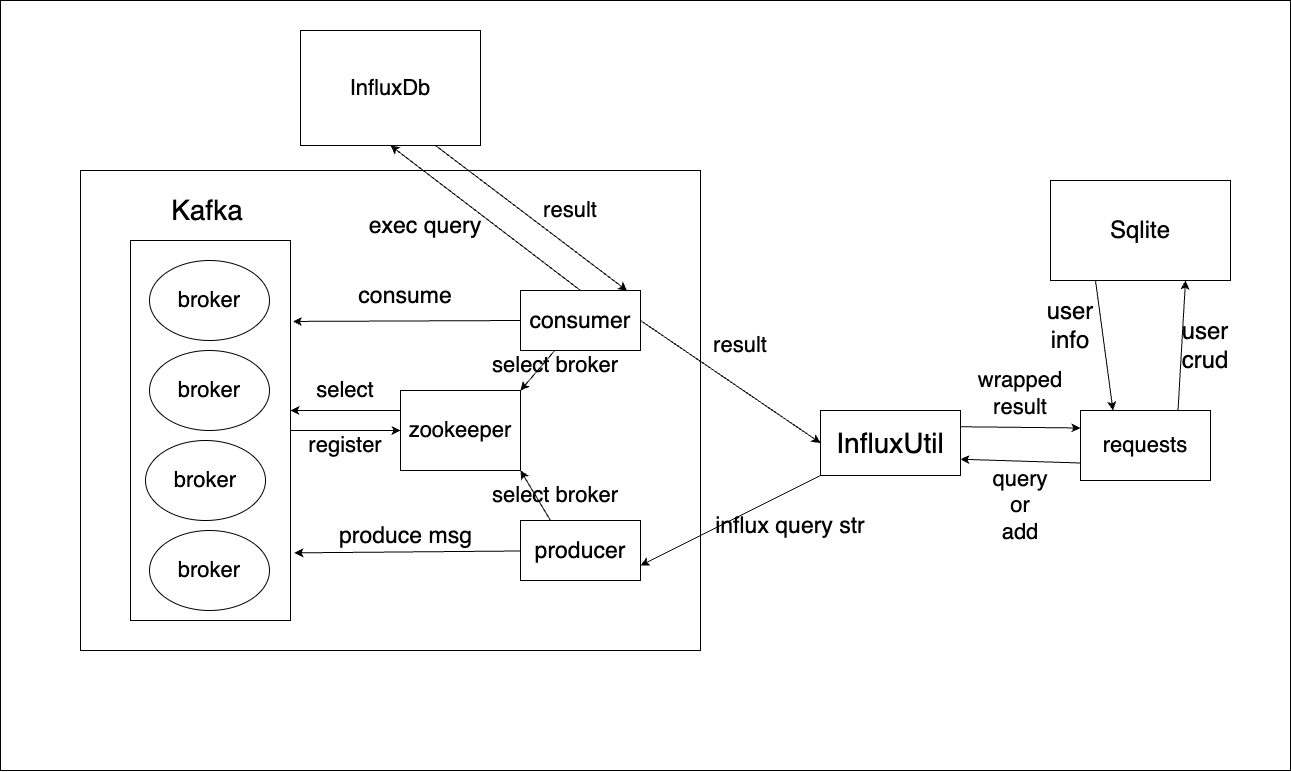
\includegraphics[width=0.8\linewidth]{images/architecture.png}
    \caption{系统架构图}
    \label{fig:architecture}
\end{figure}

下面对该系统架构图\ref{fig:architecture}进行具体阐述和解释。

\subsection{数据库设计}

根据系统架构图\ref{fig:architecture}所示,系统中的数据存储部分主要采用了以下两种数据库:

\begin{itemize}[nosep]
    \item \textbf{InfluxDB}:用于存储时序数据。InfluxDB是一种高效的时序数据库,专门用于处理时间序列数据(如传感器数据、监控数据等)。其高性能的写入和查询能力,非常适合存储和分析大量的时序数据。
    \item \textbf{SQLite}:用于存储用户信息数据。SQLite是一种轻量级的关系型数据库,适用于存储用户信息、配置数据等结构化数据。其简单的架构和嵌入式特性使其非常适合在小型应用或嵌入式系统中使用。
\end{itemize}

\subsection{消息队列设计}

根据系统架构图\ref{fig:architecture}所示,消息队列采用了Kafka和Zookeeper的架构,具体实现如下:

\begin{itemize}[nosep]
    \item \textbf{Kafka}:用于消息的生产和消费。Kafka是一个分布式流处理平台,能够处理高吞吐量的实时数据流。多个Kafka的broker注册到Zookeeper注册中心中,确保系统的可扩展性和高可用性。
    \item \textbf{Zookeeper}:作为注册中心,负责管理Kafka集群中的元数据,帮助各主题的consumer和producer找到broker进行消息的生产和消费。
\end{itemize}

\subsection{系统交互流程}

根据系统架构图\ref{fig:architecture}所示,在整个系统中,消息的生产和消费流程如下:

\begin{enumerate}[nosep]
    \item \textbf{消息生产}:Producer通过Zookeeper找到对应的Kafka broker,将消息发送到指定的主题。
    \item \textbf{消息消费}:Consumer通过Zookeeper找到对应的Kafka broker,从指定的主题中消费消息。Consumer负责与InfluxDB进行交互,在数据库中执行由InfluxUtil封装好的Influx查询串,然后返回操作结果。
    \item \textbf{结果处理}:InfluxUtil是Spring后端项目中的一个组件,负责对查询结果进行封装,然后返回给前端。
\end{enumerate}

对于用户信息数据,前端直接通过API与SQLite数据库进行交互,执行用户信息相关的增删改查操作,而不经过消息队列。这种直接访问方式简化了用户信息处理的流程,提高了系统响应速度。

\subsection{组件功能}

\begin{itemize}[nosep]
    \item \textbf{InfluxUtil}:一个Spring后端项目中的组件,负责封装InfluxDB的查询操作。它接收查询请求,执行相应的查询,并对结果进行封装,最后将封装后的结果返回给前端。该组件有效地简化了与InfluxDB的交互过程,提高了代码的可维护性和可读性。
\end{itemize}

根据系统架构图\ref{fig:architecture}所示,通过采用InfluxDB和SQLite相结合的数据库设计,以及Kafka和Zookeeper的消息队列架构,系统能够高效地处理和存储时序数据和用户信息数据。这样的设计不仅保证了数据的实时性和一致性,还提供了良好的扩展性和稳定性。

\let\cleardoublepage\clearpage
\chapter{详细设计}

本章节对各个部分设计进行具体阐述和分析,从为什么使用某个组件,到某个组件的原理,再到具体使用该组件的设计和开发过程进行介绍。

\section{数据库设计与开发}

\subsection{InfluxDB数据库设计}

本系统是一个专注于处理海量来自学生、教师佩戴的智能设备所发出的时序数据,本系统采用了InfluxDB这个数据库来处理这些时序数据。根据\cite{InfluxDB维基百科}记录的习惯详细,InfluxDB是一个由InfluxData\cite{InfluxDB维基百科}开发的开源时序型数据库,着力于高性能地查询与存储时序型数据。InfluxDB被广泛应用于存储系统的监控数据,IoT行业\cite{redhat-IoT}的实时数据等场景。下面将阐述InfluxDB的原理并对本系统中的设计进行详细阐述。

\subsubsection{InfluxDB原理分析}

InfluxDB是一款专门用于处理时序数据的TSDB,每条数据都以时间戳作为主键,便于高效地处理时间数据。InfluxDB底层的数据结构不同与常见的关系型数据如MySQL,它采用的是TSM\cite{tencentLSMTSM},TSM是一种类似于LSM\cite{tencentLSMTSM}的存储结构。LSM是一种广泛被应用于NOSQL\cite{mongodbWhatNoSQL}的存储结构,LSM树核心思想的核心就是放弃部分读能力,换取写入的最大化能力。这也就是LSM在某些情况比B+树\cite{oiwikix6811Wiki}更合适的原因,由于在本系统中,对于智能设备数据操作的场景一直需要大量的写入,而不需要很多读取和修改操作,所以使用LSM这种结构是相当合适的,性能会比B+树快上不少。而InfluxDB所采用的TSM就是一种类似于LSM的结构,对于TSM的存储流程,可以从\cite{InfluxDB官方文档}得到一些解释:批量的数据将会被写或更新到缓存中并将操作写入日志中以确保在宕机之类的情况发生时数据的可恢复性。缓存中的数据按键值有序地被组织好,且会周期性地写入到磁盘中,以TSM文件的格式存储着。

\subsubsection{使用InfluxDB设计和开发}

对于本系统,需要处理的就是多个不同的智能设备所发出的时序数据。本系统对每个类型的智能设备数据设计单独的measurement,将它们存储到同一个名为equipments的bucket中,以保留时间为3天,分片时间长度为1小时的数据归档策略,将该bucket的数据周期性地归档到另一个名为equipments-downsample的bucket中,该bucket的数据保留时间为30天,分片时间长度为1天。

系统使用equipments的数据进行可视化显示,使用equipments-downsample中的数据进行后续的统计分析。对于measurement的具体设计,每个measurement都以时间戳为主键,以每个用户的ID作为tag,智能设备所发出的其它信息则作为field。在查询时,根据数据类型、用户的ID以及时间信息即可查出相关数据。如图\ref{fig:bucket}所示,显示的即为具体的bucket创建语句。

\begin{figure}[htb]
    \centering
    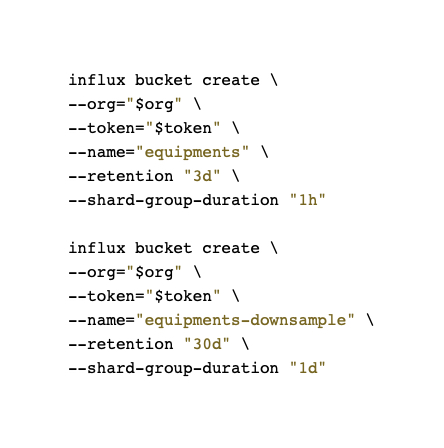
\includegraphics[width=0.8\linewidth]{images/code-bucket.jpeg}
    \caption{bucket创建语句}
    \label{fig:bucket}
\end{figure}

% \begin{lstlisting}[language=bash]
% influx bucket create \
% --org="$org" \
% --token="$token" \
% --name="equipments" \
% --retention "3d" \
% --shard-group-duration "1h"

% influx bucket create \
% --org="$org" \
% --token="$token" \
% --name="equipments-downsample" \
% --retention "30d" \
% --shard-group-duration "1d"
% \end{lstlisting}

这里通过influx命令行和influx数据操作脚本语句进行操作,其中org和token为相关组织和密钥,name为bucket名称,retention为数据保存时间,shard-group-duration为分片时间长度。

如图\ref{fig:influx-object}显示的代码,是关于人体血压的数据结构:

\begin{figure}[htb]
    \centering
    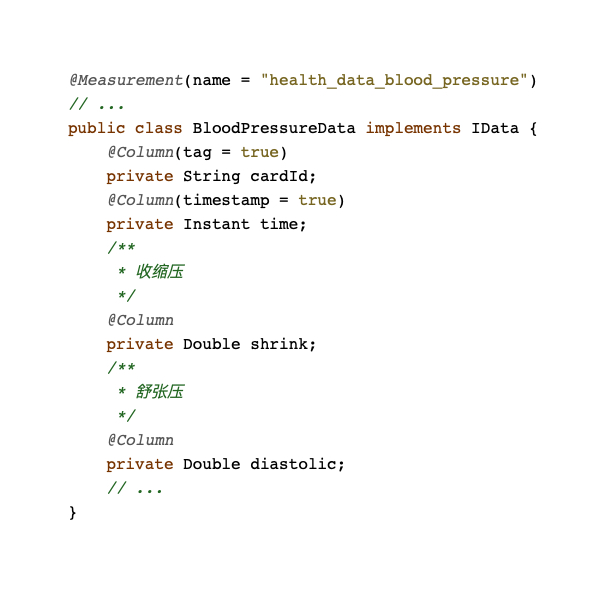
\includegraphics[width=0.8\linewidth]{images/code-object.jpeg}
    \caption{人体血压的数据结构}
    \label{fig:influx-object}
\end{figure}

% \begin{lstlisting}[language=java]
% @Measurement(name = "health_data_blood_pressure")
% // ...
% public class BloodPressureData implements IData {
%     @Column(tag = true)
%     private String cardId;
%     @Column(timestamp = true)
%     private Instant time;
%     /**
%      * 收缩压
%      */
%     @Column
%     private Double shrink;
%     /**
%      * 舒张压
%      */
%     @Column
%     private Double diastolic;
%     // ...
% }
% \end{lstlisting}

其中@Measurement中的name字段指定了measurement,@Column中的tag字段指定了cardId,即用户id作为tag,@Column中的timestamp字段指定了时间戳,即数据的主键,其它@Column注解的字段即为field。

\subsection{Sqlite数据库设计}

本系统采用Sqlite对用户相关的信息数据进行存储,下面将从为什么使用Sqlite以及使用Sqlite设计和开发进行阐述。

\subsubsection{为什么使用Sqlite}

Sqlite作为一款优秀的嵌入式数据库,被广泛运用于各种领域。根据\cite{SQLite官方文档}介绍,Sqlite不像其他的数据库,它没有一个单独的数据库服务进程,它直接通过磁盘文件进行读写操作。一个完整的数据库所包含的表、索引、触发器等元素都被存在一个单独的磁盘文件中。但是为什么Sqlite而不是其他数据库呢?

本智慧教育系统集中处理的是时序数据,而对于其它数据的需求较少,仅有用户信息这一数据需要进行存储,同时,没有事务相关的问题需要考虑,使用Sqlite这样轻便的嵌入式数据库非常合适。相比于其他关系型的数据库,如MySQL、PostgreSQL等,Sqlite的优势在于更加便于开发和使用,同时对系统的压力更小,占用的内存更低。在系统中可以划分更多内存给InfluxDB相关的服务使用,充分利用了系统。

\subsubsection{使用Sqlite设计和开发}

Sqlite对于开发者来说,不需要考虑如何具体去运行相关的数据库服务,只需要考虑如何设计数据库。在本系统中,需要存储的只有用户信息这个数据。以用户的ID作为主键即可,本系统用户表相关字段及其含义设计如下:

\begin{itemize}[nosep]
    \item \texttt{card\_id}:用于存储用户的卡号ID,作为用户的一个标识信息。
    \item \texttt{class\_id}:用于存储用户所属的班级ID,方便进行班级相关的管理。
    \item \texttt{college}:用于存储用户所属的学院信息,帮助分类和管理用户。
    \item \texttt{department}:用于存储用户所属的系信息,进一步细化学院下的分类。
    \item \texttt{major}:用于存储用户的专业信息,有助于专业相关的统计和管理。
    \item \texttt{name}:用于存储用户的姓名,作为基本的个人信息。
    \item \texttt{id}:用户的唯一标识符,是该表的主键,保证每个用户的唯一性。
\end{itemize}

该表用于存储用户的基本信息,包括学术相关信息(班级、学院、系、专业)和个人信息(卡号、姓名)。\texttt{id} 列是表的主键,用于唯一标识每一个用户。其他字段(\texttt{card\_id}, \texttt{class\_id}, \texttt{college}, \texttt{department}, \texttt{major}, \texttt{name})都是字符串类型,长度不超过255字符,用于存储用户的详细信息。

\section{后端设计与开发}
\subsection{后端技术选型}

本系统在后端使用了Java作为主要开发语言,Python作为辅助开发语言,采用了以Spring为主导的架构,其依赖项主要包含如下这些:

\begin{itemize}[nosep]
    \item 消息队列Kafka
    \item 注册中心Zookeeper
    \item 测试组件Spock
    \item 部署工具Docker
\end{itemize}

消息队列Kafka用于解决高并发问题。当大量请求同时打到服务器时,需要一个类似缓冲器的组件来暂存这些请求,防止它们一次性涌入数据库,从而造成系统过载。Kafka充当了这个缓冲器,通过高效的消息队列机制,分散和调节流量,确保系统的稳定运行。

注册中心Zookeeper是Kafka的关键依赖项。它为Kafka提供了服务发现、负载均衡和故障转移等功能。Zookeeper通过维护Kafka集群的元数据,帮助管理分布式环境中的节点协调和领导选举,从而确保Kafka集群的高可用性和一致性。

测试组件Spock是一个强大的测试框架,主要用于编写单元测试。Spock提供了简洁而直观的语法,使得编写和维护测试代码变得非常方便。使用Spock,开发人员可以高效地创建详细的测试用例,覆盖各种场景,从而减少调试时间,提高代码质量和可靠性。

部署工具Docker极大简化了应用程序的部署过程。Docker可以将应用程序及其所有依赖项打包成一个可移植的容器,然后在任何环境中快速部署。通过一键部署开发环境,Docker减少了大量的环境搭建时间,提高了开发和运维效率。

通过Kafka的高并发处理能力、Zookeeper的协调管理功能、Spock的高效测试支持,以及Docker的简便部署流程,能够构建出更加可靠、可扩展且易于维护的系统。

\subsection{后台Spring项目结构设计}

本系统后台采用Spring框架进行构建,项目由多个模块组成,每个模块都有特定的作用和相互关联。以下是对各个模块的详细阐述及其之间的关系。

\begin{itemize}[nosep]
    \item \textbf{config模块}:配置模块,用于配置跨域资源和Kafka相关设置。
    \item \textbf{controlle模块}:控制器模块,用于提供高性能接口。
    \item \textbf{dao模块}:数据操作模块,dao即数据访问对象,用于操作数据库。
    \item \textbf{exception模块}:异常处理模块,捕获并处理应用程序中未捕获的异常,提供统一的错误响应。
    \item \textbf{mq模块}:消息队列模块,用于生产和消费消息。
    \item \textbf{pojo模块}:类型模块,存储系统中所使用到的各个类对象。
    \item \textbf{type模块}:枚举模块,定义数据类型的标识。
    \item \textbf{util模块}:实用工具模块,用于提供统一公用的方法。
\end{itemize}

配置模块提供了跨域请求和Kafka的配置信息,确保应用能够正确处理前端请求和消息队列操作。控制器模块依赖DAO模块来访问和操作数据库中的数据。它们还使用服务层(如消息队列模块)来处理复杂的业务逻辑和消息队列操作。DAO模块直接与数据库交互,提供数据持久化功能。异常处理模块确保应用程序中的错误能够被统一处理,提高系统的稳定性和用户体验。消息队列模块负责Kafka消息的生产和消费,与配置模块中的Kafka配置紧密相关。POJO模块定义了应用程序中的数据模型,这些模型在控制器、服务、DAO等层中被广泛使用。类型模块定义了常量和枚举类型,用于确保代码的可读性和维护性。实用工具模块提供了一些常用的功能,如与InfluxDB的交互,帮助简化代码并提高复用性。

通过以上设计,各个模块协同工作,形成一个完整的Spring应用程序,处理用户请求、数据存储、消息队列操作和异常处理等任务。

\subsection{实现高可用接口的设计思路}

针对时序数据这一海量数据的处理,系统性能功能至关重要。学生和教师所使用的智能设备在不断产生数据的同时,系统需要应对高峰期的数据涌入,以避免对数据库造成过大压力和系统崩溃的风险。在硬件条件受限的情况下,高并发场景可能导致系统CPU负载过高,最终影响系统的稳定性和可靠性。本系统通过消息队列Kafka来应对高并发场景,实现高可用。

Kafka是一个分布式的消息系统,在本系统中通过Zookeeper来进行协调管理,确保消息的可靠生产和消费。下面分别从为什么使用Kafka、Kafka原理分析、Kafka在本项目中的设计三方面具体参数详细设计思路。

\subsubsection{为什么使用Kafka}

Kafka提供了高性能、可靠性、可扩展性和灵活性等优点,使得它成为构建实时数据处理系统和分布式消息传递系统的理想选择。相比于其他消息队列,Kafka对流式处理、分布式系统的支持更好,且其社区支持和成熟度相对于其他消息队列更好,稳定性更高。相比于其他组件如RabbitMQ,在吞吐量上,RabbitMQ比Kafka要低了一个数量级,这是kafka最大的优点,就是吞吐量高,非常适合去配合大数据类的系统来进行实时数据计算、日志采集等场景,对于本系统而言,智能设备所发出的数据是海量的,吞吐量高和强大的实时计算功能有利于高效地处理数据。另外Kafka在大数据领域的实时计算以及日志采集被大规模使用,相比于较为不成熟的RocketMQ,Kafka是事实上的标准,稳定性和可靠性更高。

\subsubsection{Kafka原理分析}

首先明确Kafka的各个节点。Kafka是一个分布式系统,它由多个节点组成,每个节点称为一个Broker。Broker之间可以进行数据的分布式存储和传输,实现数据的高可用性和水平扩展。Kafka通过主题(Topic)对数据进行组织和分类,每个主题可以分成多个分区(Partition)。分区是 Kafka中数据的基本存储单元,它们可以分布在不同的Broker上,实现数据的并行处理和负载均衡。Kafka中的数据单元称为消息(Message),每个消息由一个键值对(Key-Value)组成,包括消息的键(Key)和消息的值(Value)。消息的键用于确定消息的分区,而消息的值是实际的数据内容。

关于Kafka的存储过程,Kafka提供了生产者(Producer)和消费者(Consumer)两种角色,用于向Kafka中写入数据和从Kafka中读取数据。生产者将消息发布到指定的主题中,而消费者订阅感兴趣的主题并从中拉取消息。Kafka中的数据以日志的形式进行存储,每个分区都有一个对应的日志文件,用于顺序存储消息。消息一旦被写入到日志中就不可修改,保证了数据的持久性和不可变性。Kafka使用副本机制(Replication)来提高数据的可靠性和容错性。每个分区可以配置多个副本,这些副本分布在不同的 Broker 上,保证了数据的备份和故障恢复能力。

\subsubsection{Kafka在本项目中的设计}

Kafka是一个分布式的消息系统,在本系统中通过Zookeeper来进行协调管理,确保消息的可靠生产和消费。下面详细描述本系统中,Kafka与Zookeeper在消息消费和生产中的设计和工作原理。

消息生产者负责将消息发送到Kafka集群中的指定主题。其主要工作流程如下:

\begin{itemize}[nosep]
    \item \textbf{连接到Kafka集群}:生产者首先通过Zookeeper获取Kafka集群的元数据,包括可用的broker列表和主题的分区信息。
    \item \textbf{选择分区}:生产者根据配置的分区策略(如轮询、按键散列等)选择一个分区,将消息发送到该分区。
    \item \textbf{发送消息}:生产者将消息发送到选择的分区对应的broker,Kafka集群保证消息在分区内的顺序性。
    \item \textbf{确认消息}:生产者等待broker的确认,以确保消息成功写入。根据配置,可以是leader副本确认或所有副本确认。
\end{itemize}

消息消费者负责从Kafka集群中读取消息。其主要工作流程如下:

\begin{itemize}[nosep]
    \item \textbf{连接到Kafka集群}:消费者通过Zookeeper获取Kafka集群的元数据,包括可用的broker列表和主题的分区信息。
    \item \textbf{加入消费者组}:消费者加入一个消费者组,Zookeeper帮助协调组内的消费者,分配主题的分区给各个消费者。
    \item \textbf{拉取消息}:消费者从分配到的分区对应的broker拉取消息,Kafka支持批量拉取,提高消费效率。
    \item \textbf{提交偏移量}:消费者定期向Zookeeper提交已消费的消息偏移量,以便在故障恢复时能够从正确的位置继续消费。
\end{itemize}

通过以上设计,Kafka利用Zookeeper实现了可靠的消息生产和消费,确保了消息系统的高可用性和一致性。

\section{前端设计与开发}

下面将从技术选型、各组件的具体介绍和使用、架构设计、启动流程等方面来对前端的设计与开发继续阐述。

\subsection{技术选型}

前端使用了Html、CSS、JavaScript作为主要的开发语言,依赖了图表库Echart,请求工具Axios等组件。

ECharts是一个功能强大、交互式的图表库和浏览器数据可视化工具。它是由Apache软件基金会维护的一个免费开源项目。ECharts提供了各种各样的图表类型,包括折线图、柱状图、饼图、散点图、地图等等。它还提供了丰富的图表定制功能,例如主题、颜色、注释和交互等。在本项目中通过Echart来渲染图表库,大大减少了在前端开发所花费的时间,且生成的图表美观、稳定性好。

Axios是一个基于Promise的HTTP客户端库,可用于浏览器和Node环境。它以易于使用、功能强大和可扩展性著称,是许多开发人员的首选方案。本项目通过Axios请求后端接口,通过其简洁的API设计,大量减少了前端开发时间。

\subsection{架构设计}

数据请求与渲染过程设计如下:

页面通过Axios库向后端服务发送请求,以加载和刷新数据。具体来说,页面每隔1秒请求后台接口,包括获取最新数据的接口和指定时间范围内的数据接口。这种设计确保了数据的实时性和连续性。

\begin{itemize}[nosep]
    \item \textbf{定时请求}:
    \begin{itemize}[nosep]
        \item \textbf{最新数据接口}:每秒请求一次最新数据,确保界面上的数据是最新的。
        \item \textbf{时间范围数据接口}:每秒请求一次指定时间范围内的数据,便于数据分析和展示。
    \end{itemize}
    \item \textbf{异步监听}:
    \begin{itemize}[nosep]
        \item \textbf{成功处理}:如果请求结果的状态码为200,则表明请求成功,并将最新数据渲染到图表上。
        \item \textbf{失败处理}:如果请求失败,则重新发送请求。如果连续3次请求失败,则向用户反馈错误信息。
    \end{itemize}
\end{itemize}

为了获取不同用户数据,本系统通过URL请求参数指定不同的用户ID,界面初始化时将该ID设为全局变量,以后每次请求数据时都在请求体中包含该用户ID,从而获取到不同用户的数据。

\begin{itemize}[nosep]
    \item \textbf{URL参数}:根据URL中的请求参数获取用户ID。
    \item \textbf{全局变量}:在界面初始化时,将用户ID设为全局变量。
    \item \textbf{请求体中的用户ID}:每次请求数据时,都在请求体中包含该用户ID,以确保请求的是该用户的数据。
\end{itemize}

\let\cleardoublepage\clearpage
\chapter{软件测试与结果呈现}

本章节将介绍软件测试与结果呈现相关的内容。本项目的测试计划包括了单元测试、集成测试、接口压力测试、可视化测试,下面将具体对这四个测试的技术选型、相关实现、测试过程、测试结果等进行阐述。

\section{单元测试}

单元测试是一种软件测试方法,用来检验程序单元(软件设计的最小可测试部件)是否按照设计正确地工作。程序单元可以是一个函数、一个方法、一个类或者一个模块。单元测试的目的是发现并修复程序单元中的错误,从而提高软件的质量。

\subsection{技术选型}

后端部分采用了Spock框架用于编写单元测试,而前端无需进行单元测试。关于Spock相关的内容,在后端开发部分已经介绍的很清楚,Spock具有可读性高、灵活性、集成度高、易于扩展、内置Mocking支持、数据驱动测试和丰富的文档和社区支持等优点,使得它成为Java开发中一个受欢迎的测试框架。在本系统中,通过Spock可以非常轻松地编写单元测试来测试来自多种类型智能设备的数据操作。

\subsection{代码实现}

Spock测试方法需要遵循given-when-then(-where)的原则,下面以开发一个测试查询数据的函数为例进行阐述,如图\ref{fig:spock}测试了查询各种类型智能设备在一段时间内所发出的数据这个方法。

\begin{figure}[htb]
    \centering
    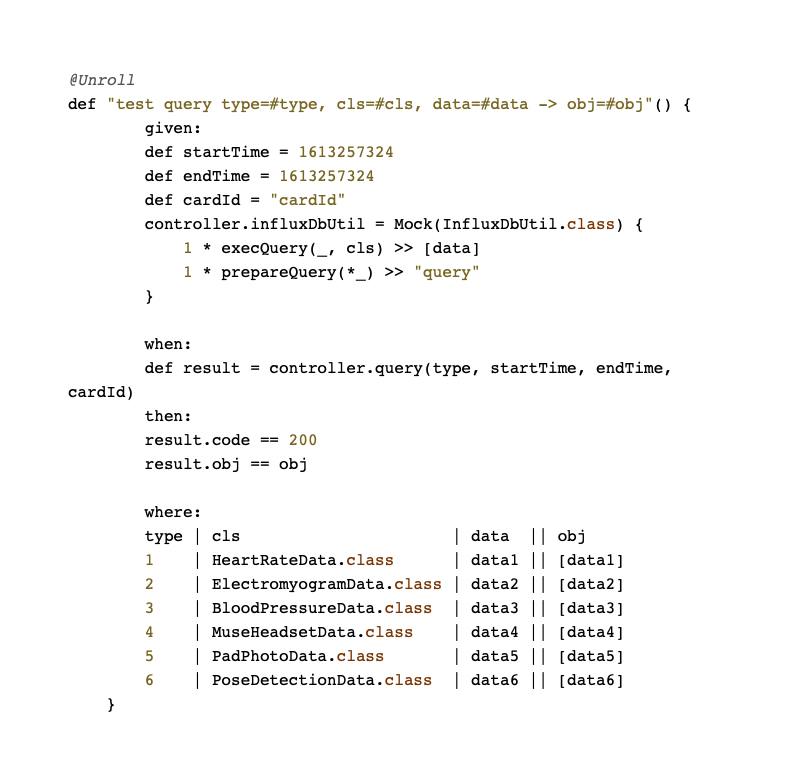
\includegraphics[width=0.8\linewidth]{images/code-spock.jpeg}
    \caption{spock单元测试示例}
    \label{fig:spock}
\end{figure}

如图\ref{fig:spock}所示,在given块中,指定了开始时间、结束时间、用户ID等信息,并且mock了相关方法;在when块中,执行了query方法进行数据查询,返回结果result;在then块中,对result进行assert判断;在where块中,加载了本系统所涉及到了6种数据以及相应的返回结果。

除了该单元测试,本系统还提供了其他多种单元测试,包括对智能设备接口函数的测试,它们均遵循given-when-then的测试结构,这里不再一一进行展示,下面将执行这些单元测试。

\subsection{测试结果}

执行所有单元测试,如图\ref{fig:spock-result}所示,所有测试均通过。

\begin{figure}[htb]
    \centering
    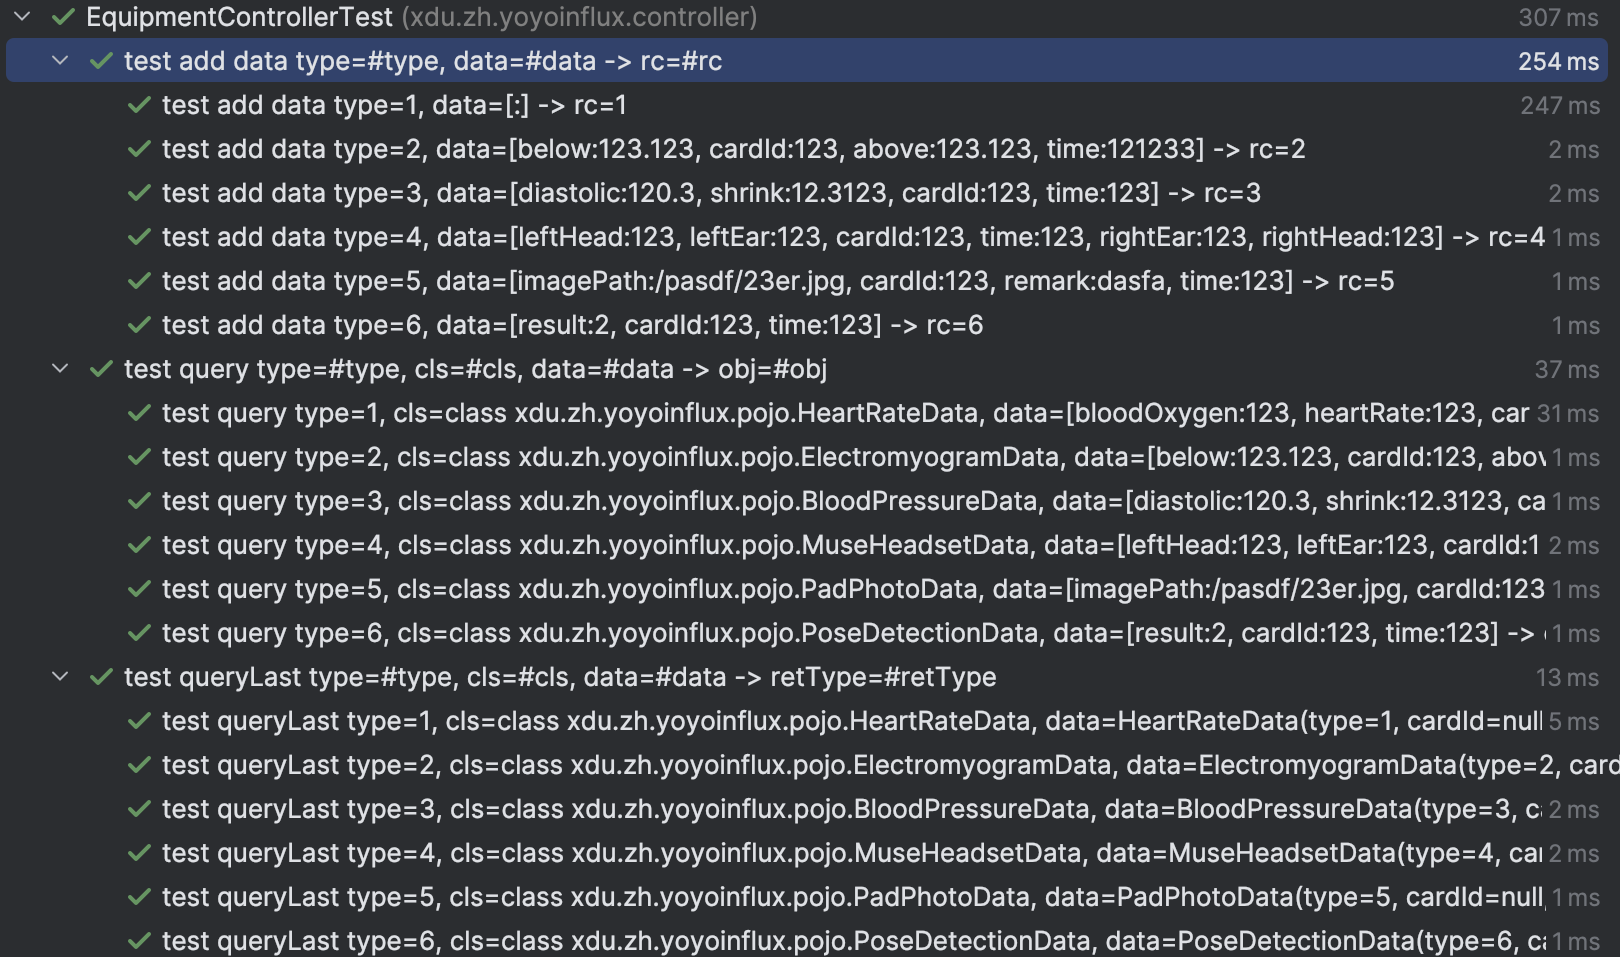
\includegraphics[width=0.8\linewidth]{yoyo-tex//images/spock-result.png}
    \caption{单元测试执行结果}
    \label{fig:spock-result}
\end{figure}

如图\ref{fig:spock-result}所示,一共包含三个测试组,分别为新增数据的接口测试、查询某段时间内的数据接口测试、查询最新数据的接口测试。每个测试组包含多组测试条件,覆盖所有测试智能设备相关数据类型。

\section{集成测试}

集成测试是一种软件测试方法,用来检验多个软件单元组合在一起是否按照设计正确地工作。软件单元可以是一个函数、一个方法、一个类或者一个模块。集成测试的目的是发现并修复多个软件单元之间的接口错误,从而提高软件的质量。

集成测试通常在单元测试之后进行。在单元测试中,每个软件单元都被单独测试,以确保其功能正确。在集成测试中,多个软件单元被组合在一起,以测试它们之间的接口是否正确。

本项目中,由于后台系统不涉及多个模块,所以没有额外编写相关测试方法,而是直接通过Rest请求来进行测试。

\subsection{技术选型}

本项目通过RestClient进行Rest集成测试,RestClient是一种通过编写遵循Rest格式的请求进行测试的测试组件。通过该组件,可以方便快捷地编写各种测试。

\subsection{代码实现}

下面以添加某种智能设备所发出的数据为例,编写相应的Rest请求测试。如图\ref{fig:rest}所示,通过环境变量baseUrl指定请求地址,通过Content-Type设定请求格式,然后在下方指定数据即可。

\begin{figure}[htb]
    \centering
    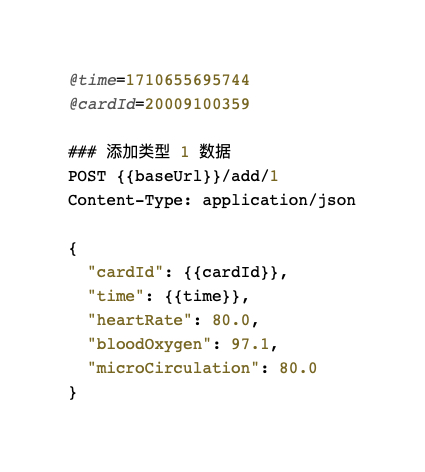
\includegraphics[width=0.8\linewidth]{images/code-rest.jpeg}
    \caption{rest请求示例}
    \label{fig:rest}
\end{figure}

除了本测试,系统对所有接口都编写了相应测试,下面对这些接口进行测试。

\subsection{测试结果}

本系统中主要涉及两大部份接口,包括智能设备和用户这两部份。对于智能设备,需要测试所有类型的数据的插入操作、查询操作,对于用户,需要测试对用户的查找和新增操作。测试结果如图\ref{fig:rest-test-result}所示。

\begin{figure}[htb]
    \centering
    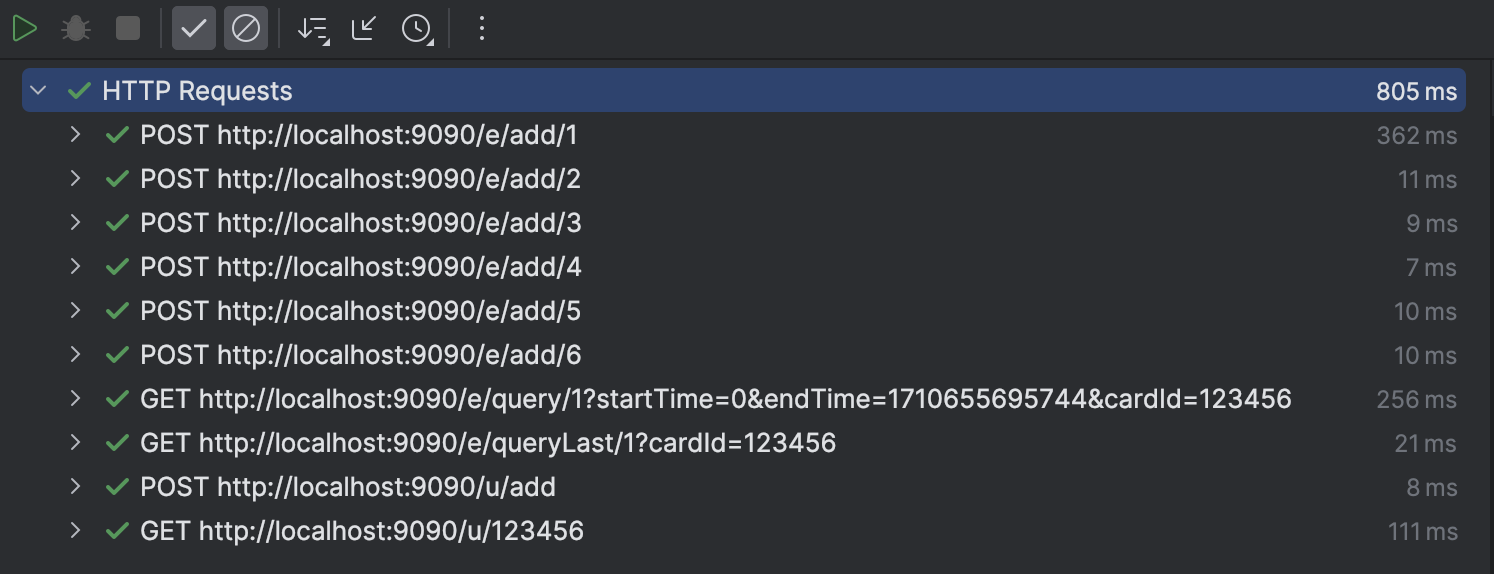
\includegraphics[width=0.75\linewidth]{yoyo-tex//images/rest-test-result.png}
    \caption{集成测试结果}
    \label{fig:rest-test-result}
\end{figure}

如图\ref{fig:rest-test-result}所示,一共进行了10个测试,分别是:

\begin{enumerate}[nosep]
    \item 新增类型 1 数据的接口测试
    \item 新增类型 2 数据的接口测试
    \item 新增类型 3 数据的接口测试
    \item 新增类型 4 数据的接口测试
    \item 新增类型 5 数据的接口测试
    \item 新增类型 6 数据的接口测试
    \item 查询某段时间内的数据的接口测试
    \item 查询最新数据的接口测试
    \item 添加新用户的接口测试
    \item 查询用户信息的接口测试
\end{enumerate}

\section{接口压力测试}

\subsection{技术选型}

本项目通过Jmeter进行接口压力测试。JMeter是一个开源的Java应用程序,用于负载测试和性能测试。它可以模拟大量用户访问各种应用程序、服务器和协议。JMeter提供了一个丰富的用户界面,用户可以配置测试计划、执行负载测试并分析测试结果。

本系统主要的压力来源于大量的数据查询操作,CPU将会是主要的性能瓶颈。因此本次测试是针对本系统数据查询接口服务进行压力测试,找到在特定硬件环境下,本系统的合适并发数。

\subsection{测试环境}

如表格\ref{tab:jmeter-test-env}所示,显示的是本次压力测试的硬件环境。

\begin{table}[htb]
    \centering
    \caption{测试环境}
    \begin{tabular}{cccc}\hline
         主机用途     & OS & CPU & 内存 \\\hline
         模拟用户请求 & MacOS & 8 & 8G \\\hline
    \end{tabular}
    \label{tab:jmeter-test-env}
\end{table}

本次测试在一台CPU数为8,内存容量为8G的MacOS系统上完成,主机用途是模拟用户请求。

\subsection{测试指标}

\begin{table}[htb]
    \centering
    \caption{测试指标}
    \begin{tabular}{cccccccc}\hline
         并发数 & 持续运行时间 & 平均响应时间  & 成功率 \\\hline
         500    & 1min       & \<1s &    90\% \\\hline
         1000   & 1min       & \<1s &	90\% \\\hline
         1250   & 1min       & \<1s &    90\% \\\hline
         1500  & 1min       & \<1s &	90\% \\\hline
    \end{tabular}
    \label{tab:jmeter-test-aim}
\end{table}

测试指标如表格\ref{tab:jmeter-test-aim}所示。本次测试将并发数从500逐步增加到1000,1250,最大到1500,每次并发请求均持续运行1分钟,根据\cite{压力测试核心性能指标及行业标准}压力测试核心性能指标及行业标准,要求成功率大于等于90\%,平均响应时间小于1s。

\subsection{测试过程}

启动JMeter,对数据查询接口进行压力测试,分别测试500、1000、1250、1500个线程,即模拟这些数目的用户并发,同时将并发持续时间设为1分钟。

\subsection{测试结果}

如表\ref{tab:performance-results-500},表\ref{tab:performance-results-1000},表\ref{tab:performance-results-1250},表\ref{tab:performance-results-1500},所示,分别为测试500、1000、1250、1500个线程时得到的结果。

如下是Jmeter测试结果的一些参数解释:

\begin{enumerate}[nosep]
    \item \textbf{Samples}: 总并发用例数。
    \item \textbf{Average}: 平均响应时间。
    \item \textbf{Min}: 最小响应时间。
    \item \textbf{Max}: 最大响应时间。
    \item \textbf{Error}: 错误率, 为错误的请求的数量除以请求的总数。
    \item \textbf{Throughput}: 吞吐量,即表示每秒完成的请求数。
\end{enumerate}

当并发数为500时,测试结果如表\ref{tab:performance-results-500}所示。平均响应时间为707ms,错误率为0\%,达到指标要求。

\begin{table}[htb]
\centering
\caption{Performance Test Results - 500}
\begin{tabular}{lrrrrrrrrrr}\hline
\toprule
\textbf{\# Samples} & \textbf{Average (ms)} & \textbf{Min (ms)} & \textbf{Max (ms)} & \textbf{Error \%} & \textbf{Throughput(req/sec)} \\\hline
\midrule
30000&707&7&3974&0.000\%&648.48039\\\hline
\bottomrule
\end{tabular}
\label{tab:performance-results-500}
\end{table}

当并发数为1000时,测试结果如表\ref{tab:performance-results-1000}所示。平均响应时间为943ms,错误率为8.608\%,达到指标要求。

\begin{table}[htb]
\centering
\caption{Performance Test Results - 1000}
\begin{tabular}{lrrrrrrrrrr}\hline
\toprule
\textbf{\# Samples} & \textbf{Average (ms)} & \textbf{Min (ms)} & \textbf{Max (ms)} & \textbf{Error \%} & \textbf{Throughput(req/sec)} \\\hline
\midrule
60000&943&0&4852&8.608\%&873.08286 \\\hline
\bottomrule
\end{tabular}
\label{tab:performance-results-1000}
\end{table}

当并发数为1250时,测试结果如表\ref{tab:performance-results-1250}所示。平均响应时间为2092ms,错误率为4.983\%,未达到指标要求。同时可以发现吞吐量开始下降,证明1250的并发请求量开始对系统造成较大压力,虽然错误率达标,但是不如并发数为1000时的吞吐量表现。

\begin{table}[htb]
\caption{Performance Test Results - 1250}
\centering
\begin{tabular}{lrrrrrrrrrr}\hline
\toprule
\textbf{\# Samples} & \textbf{Average (ms)} & \textbf{Min (ms)} & \textbf{Max (ms)} & \textbf{Error \%} & \textbf{Throughput(req/sec)} \\\hline
\midrule
75000&2092&0&6461&4.983\%&555.05806\\\hline
\bottomrule
\end{tabular}
\label{tab:performance-results-1250}
\end{table}

当并发数为1500时,测试结果如表\ref{tab:performance-results-1500}所示。平均响应时间为1678ms,错误率为15.198\%,未达到指标要求。可以发现在并发量为1500的情况下,错误率大幅提升,CPU占用率过大无法处理过多请求。

\begin{table}[htb!]
\caption{Performance Test Results - 1500}
\centering
\begin{tabular}{lrrrrrrrrrr}\hline
\toprule
\textbf{\# Samples} & \textbf{Average (ms)} & \textbf{Min (ms)} & \textbf{Max (ms)} & \textbf{Error \%} & \textbf{Throughput(req/sec)} \\\hline
\midrule
90000 & 1678 & 0 & 18892 & 15.198\% & 786.05366 \\\hline
\bottomrule
\end{tabular}
\label{tab:performance-results-1500}
\end{table}

综上所述,在CPU数为8,内存容量为8G的硬件条件下,将并发量控制在1000以内,可以较好地处理前台的数据请求操作。

\section{可视化测试}

如图\ref{fig:result1}及\ref{fig:result2}、\ref{fig:result3}所示,前后台运行状态良好,消费者正常消费消息,前台成功请求到后台数据,各个图表运行正常,图表数据动态进行显示。下面对各个结果进行详细地解释。

\begin{figure}[htb]
    \centering
    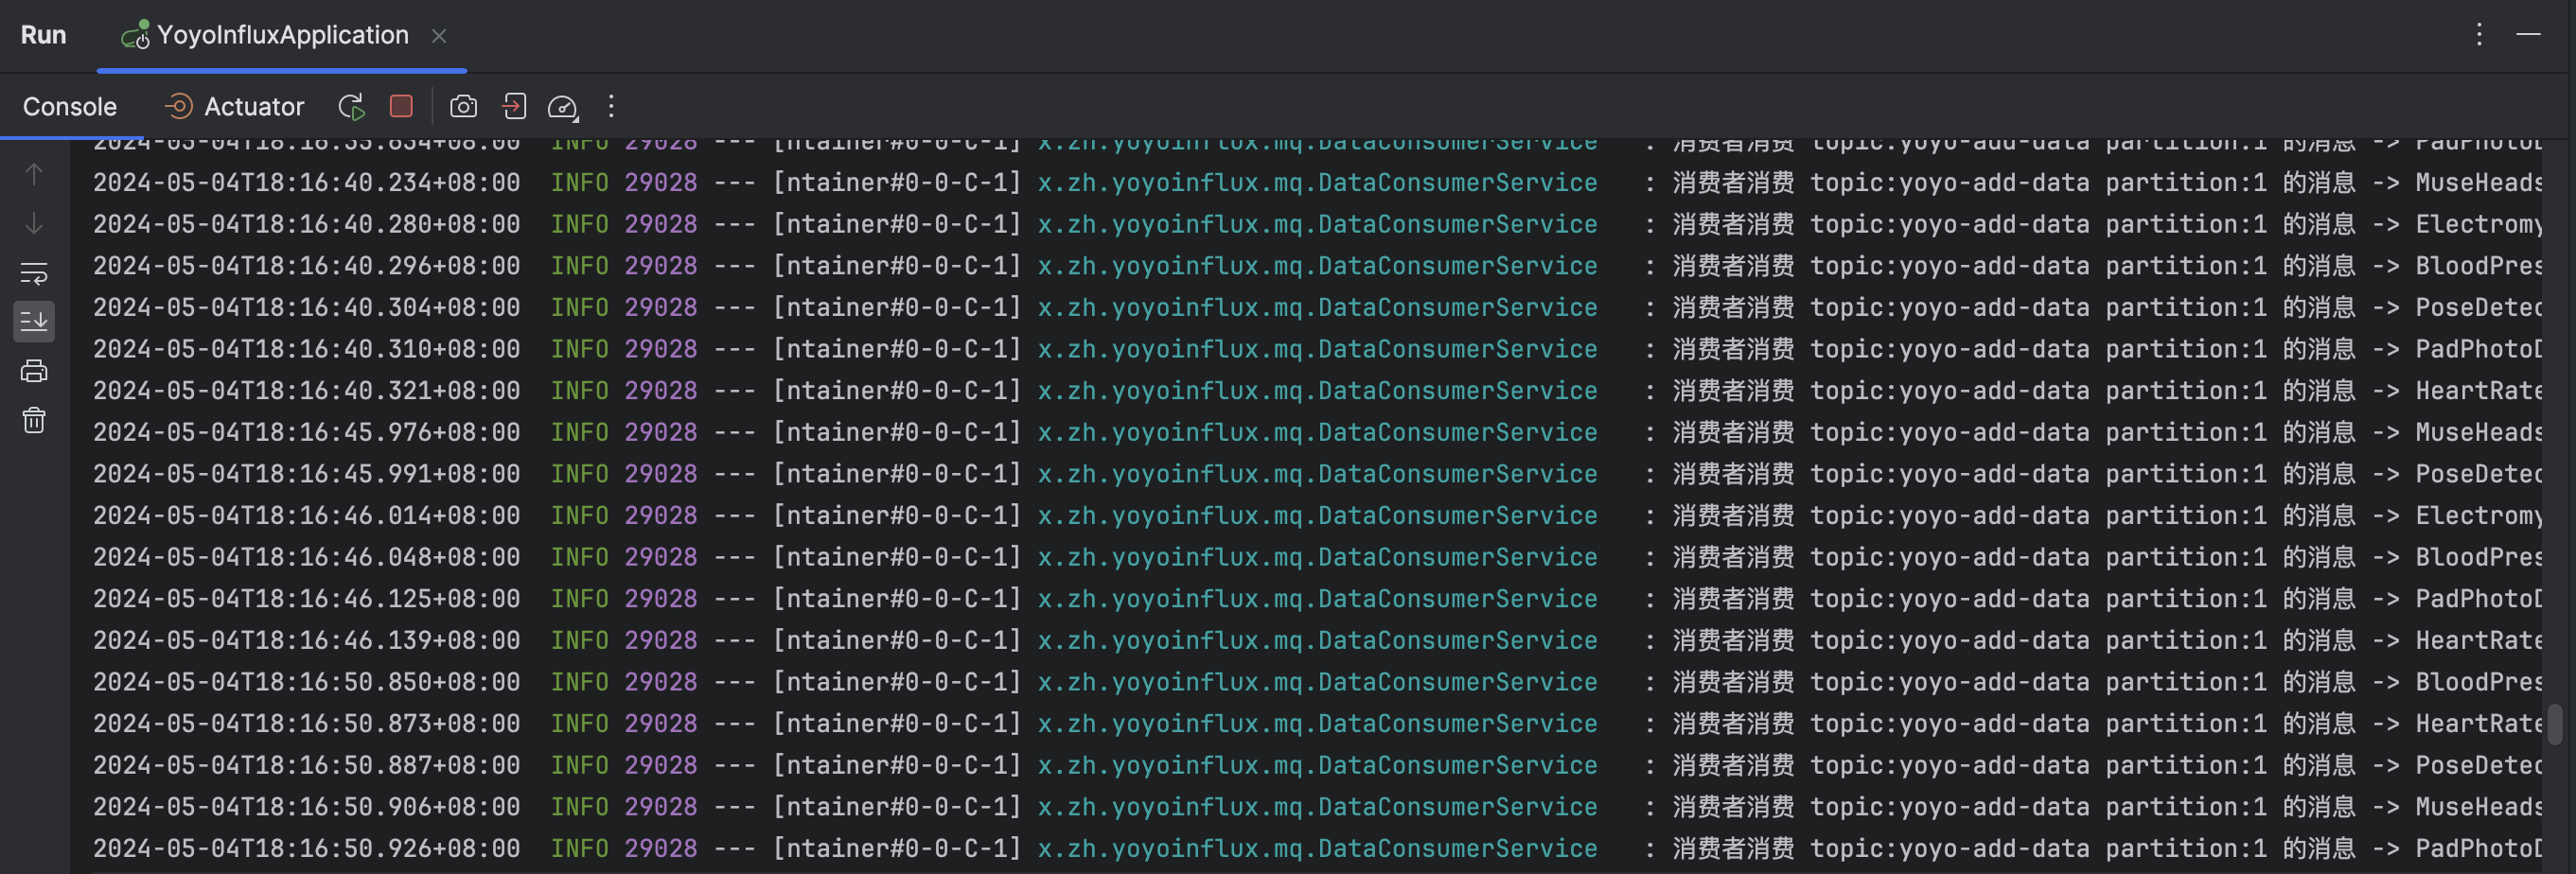
\includegraphics[width=0.8\linewidth]{images/result1.png}
    \caption{后台运行效果}
    \label{fig:result1}
\end{figure}

如图\ref{fig:result1}所示,启动后台应用程序,并启动智能设备数据模拟生成器,控制台打印日志。每行显示的是Kafka消费者的消费信息,表面系统正常接收来自数据生成器的请求,向数据库插入数据,以下是对消费信息的具体解释,根据图\ref{fig:result1}中的一条消费消息进行分析,该日志消息从左到右的显示的信息如下:

\begin{itemize}[nosep]
    \item \textbf{时间戳}:表示日志生成的日期和时间。
    \item \textbf{日志级别}:此处为信息级别。其他日志级别包括DEBUG、WARN、ERROR等。
    \item \textbf{进程ID}:生成日志消息的进程标识符。
    \item \textbf{线程}:生成日志条目的线程,此处是消费者容器线程
    \item \textbf{记录器名称}:\texttt{x.zh.yoyoinflux.mq.DataConsumerService} - 记录器的完全限定类名。在此情况下,表示\texttt{DataConsumerService}类,位于\texttt{x.zh.yoyoinflux.mq}包中。
    \item \textbf{消息}:消费者正在消费某个主题下某个分区的消息。
\end{itemize}

总结来说,这条日志消息表明,一个Kafka消费者正在消费某个主题中某个分区的一条消息。

下面开始测试前台可视化的运行效果,如图\ref{fig:result2}和图\ref{fig:result3}。

\begin{figure}[htb]
    \centering
    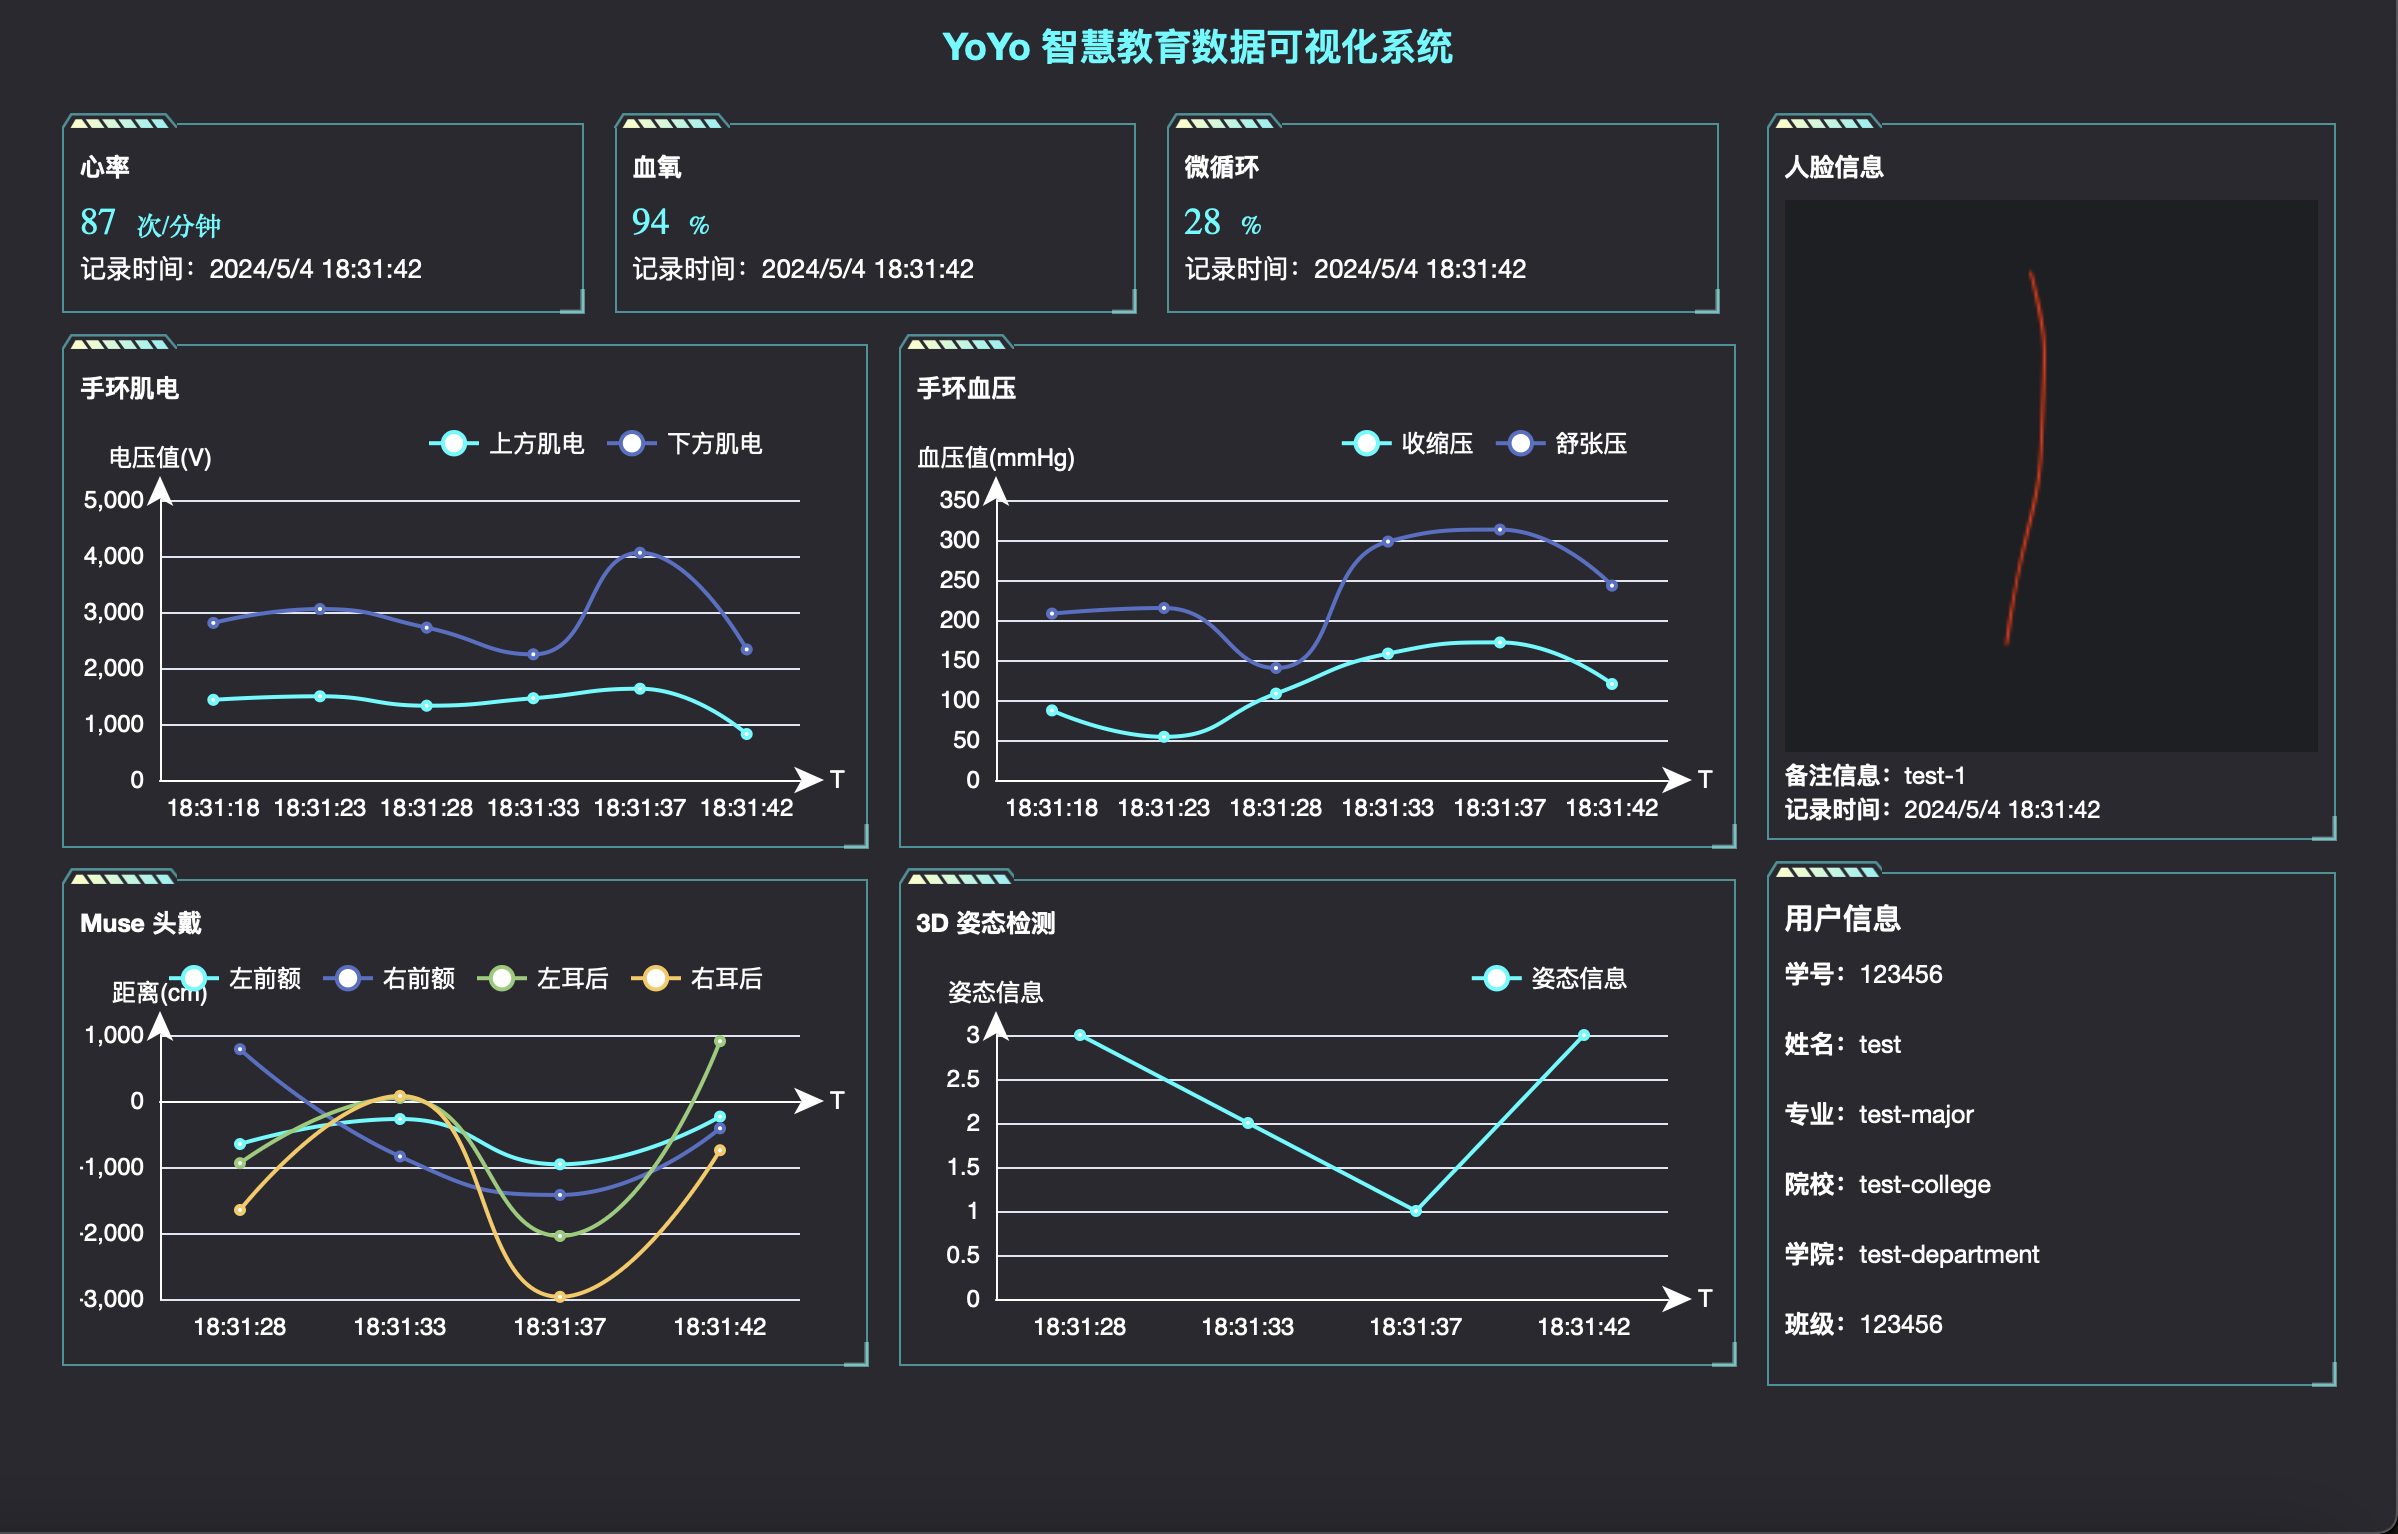
\includegraphics[width=0.9\linewidth]{images/result2.png}
    \caption{前台运行效果1}
    \label{fig:result2}
\end{figure}

如图\ref{fig:result1},展示了如下信息:

\begin{enumerate}[nosep]
    \item \textbf{心率(Heart Rate)}:
    \begin{itemize}[nosep]
        \item 显示当前心率为87次/分钟,记录时间为2024/5/4 18:31:42。
        \item 用途:监测学生的实时心率,以评估其身体健康状态或情绪波动。
    \end{itemize}

    \item \textbf{血氧(Blood Oxygen)}:
    \begin{itemize}[nosep]
        \item 显示血氧饱和度为94\%,记录时间为2024/5/4 18:31:42。
        \item 用途:检查学生的血氧水平,以了解其呼吸状况和身体供氧情况。
    \end{itemize}

    \item \textbf{微循环(Microcirculation)}:
    \begin{itemize}[nosep]
        \item 显示微循环指数为28\%,记录时间为2024/5/4 18:31:42。
        \item 用途:评估学生的微循环状况,可能用于分析其疲劳程度或身体健康。
    \end{itemize}

    \item \textbf{手环肌电(EMG from Wristband)}:
    \begin{itemize}[nosep]
        \item 图表显示了上方肌电和下方肌电的电压值随时间的变化。
        \item 用途:监控学生手部肌肉活动,可能用于分析其运动状态或应力水平。
    \end{itemize}

    \item \textbf{手环血压(Blood Pressure from Wristband)}:
    \begin{itemize}[nosep]
        \item 图表显示了收缩压和舒张压随时间的变化,单位为mmHg。
        \item 用途:实时监测学生的血压水平,以评估其心血管健康状况。
    \end{itemize}

    \item \textbf{Muse 头戴(Muse Headband)}:
    \begin{itemize}[nosep]
        \item 图表展示了左前额、右前额、左耳后和右耳后的距离随时间的变化,单位为cm。
        \item 用途:跟踪学生头部的位置和运动,可能用于分析其专注度或姿势。
    \end{itemize}

    \item \textbf{3D 姿态检测(3D Posture Detection)}:
    \begin{itemize}[nosep]
        \item 图表展示了姿态信息随时间的变化。
        \item 用途:监测学生的姿态,帮助纠正不良坐姿,预防相关健康问题。
    \end{itemize}

    \item \textbf{人脸信息(Face Information)}:
    \begin{itemize}[nosep]
        \item 显示了一个简单的人脸信息图和备注信息(test-1),记录时间为2024/5/4 18:31:42。
        \item 用途:识别和记录学生的身份信息,可能用于考勤或行为分析。
    \end{itemize}

    \item \textbf{用户信息(User Information)}:
    \begin{itemize}[nosep]
        \item 展示了学号、姓名、专业、学院、学院、班级等详细信息。
        \item 用途:提供学生的基本信息,用于个性化分析和管理。
    \end{itemize}
\end{enumerate}

\clearpage

\begin{figure}[htb]
    \centering
    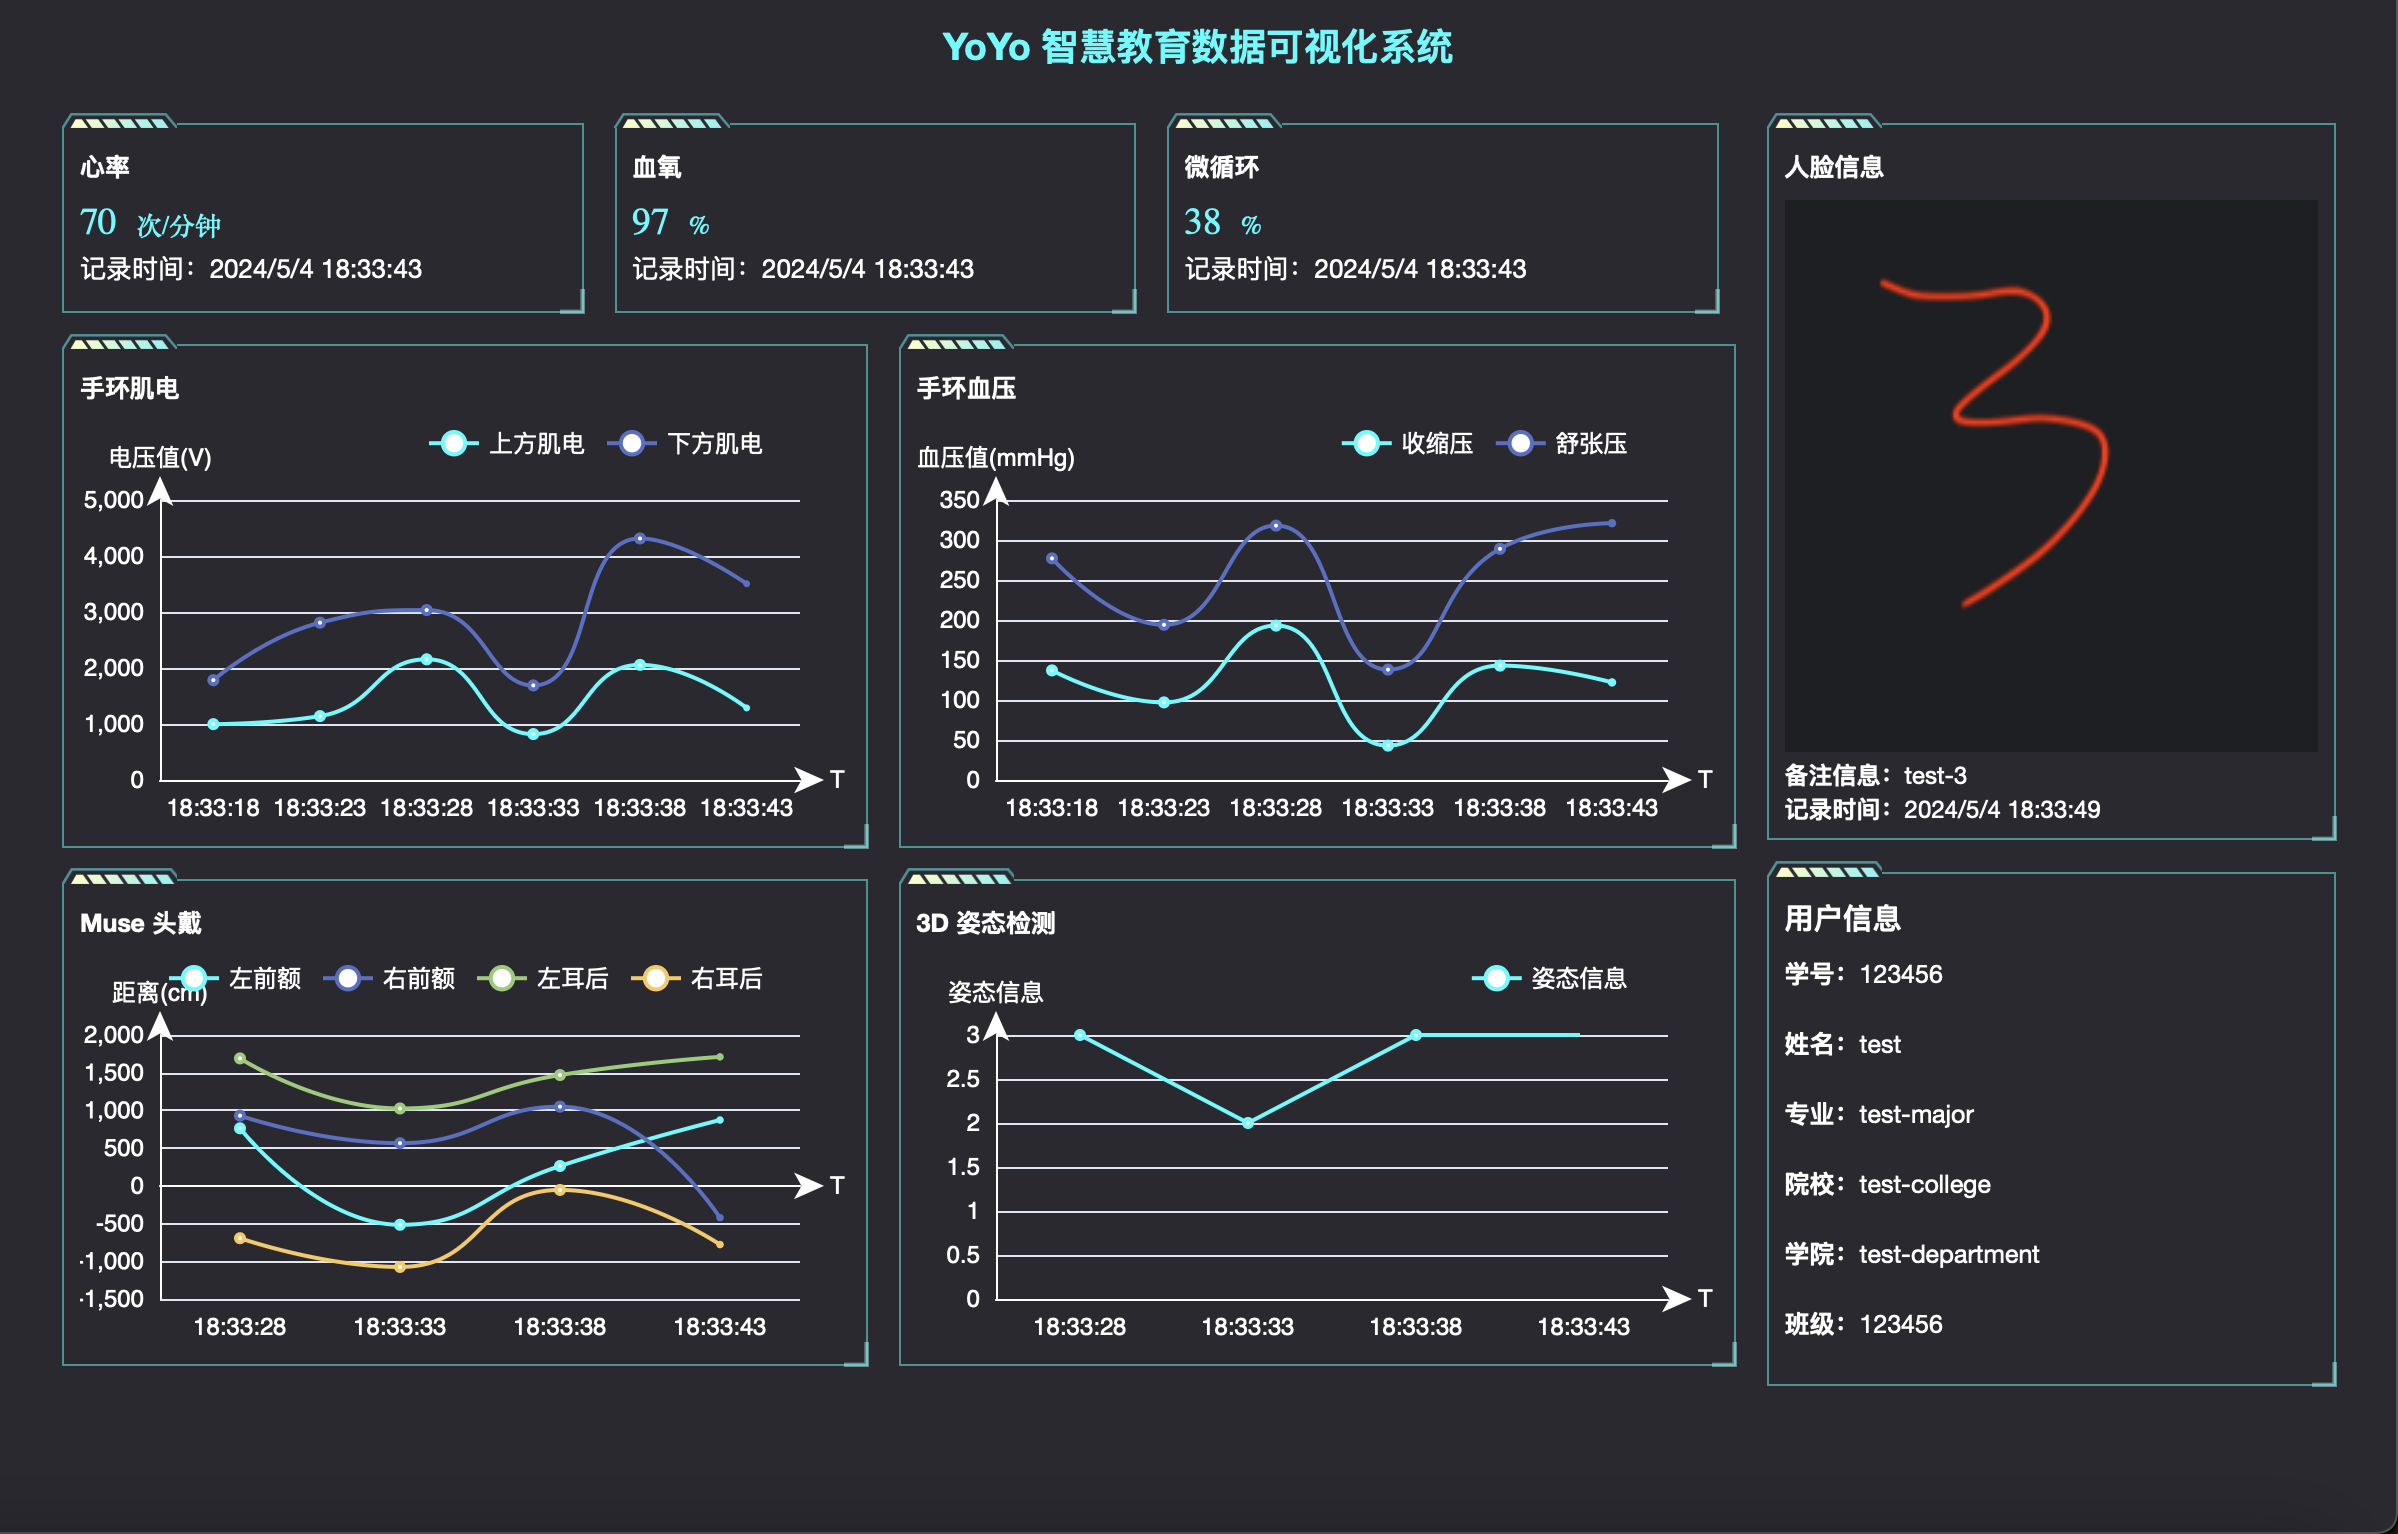
\includegraphics[width=0.9\linewidth]{images/result3.png}
    \caption{前台运行效果2}
    \label{fig:result3}
\end{figure}

如图\ref{fig:result3},该图从图\ref{fig:result1}动态变化而来,除了用户信息没有改变,其它模块包括血氧、心率、微循环、手环肌电、手环血压、Muse头戴、3D姿态检测、人脸信息等均发生动态变化,动态可视化效果正常运作。


\let\cleardoublepage\clearpage
\end{document}
